\documentclass{beamer}

\usepackage[utf8]{inputenc} % For encoding
\usepackage{graphicx}
\usepackage{amsmath}
\usepackage{amssymb}

\usepackage[T1]{fontenc}
\usepackage{booktabs}
\usepackage{multicol}
\usepackage{makecell}
\usepackage{natbib}
\usepackage{hyperref}
\usepackage{booktabs} 
\usepackage{array}    
\usepackage{tabularx}
\usepackage{tikz}

\usepackage{pgfkeys}
\usepackage{ifthen}

% \usepackage[a4paper,width=175mm,top=20mm,bottom=20mm,bindingoffset=6mm]{geometry}
\usepackage{fancyhdr}

\title{Maintenance Scheduling System}
\author{Christian Brunbjerg Jespersen}
\institute{Technical University of Denmark}
\date{\today}

\usepackage{fontspec}

% Set the main document font to Arial
\setmainfont{FiraCode Nerd Font}
\begin{document}

% Sets
\newcommand{\SetWorkOrder}[1]{W(\VarMetaTime#1)}
\newcommand{\ElementWorkOrder}{w}
\newcommand{\SetPeriod}{P(\VarMetaTime)}
\newcommand{\ElementPeriod}{p}

\newcommand{\SetResource}{R(\VarMetaTime)}
\newcommand{\ElementResource}{r}
\newcommand{\SetOperation}[2]{O_{#1}(\VarMetaTime, #2)}
\newcommand{\ElementOperation}{o}

\newcommand{\SetDays}[1]{D_{#1}(\VarMetaTime)}
\newcommand{\ElementDays}{d}
\newcommand{\SetActivity}[2]{A_{#2}(\VarMetaTime, #1)}
\newcommand{\ElementActivity}{a}

\newcommand{\SetWorkSegment}{K(\VarSupervisorAssignment{}{})}
\newcommand{\ElementWorkSegment}{k}
\newcommand{\SetTimeInstance}{I(\VarMetaTime)}
\newcommand{\ElementTimeInstance}{i}

\newcommand{\SetEvent}{E(\VarMetaTime)}
\newcommand{\ElementEvent}{e}

\newcommand{\SetScheduler}{S}
\newcommand{\ElementScheduler}{s}
\newcommand{\SetSupervisor}{Z}
\newcommand{\ElementSupervisor}{z}

\newcommand{\SetTechnician}{T(\VarMetaTime)}
\newcommand{\ElementTechnician}{t}

% Parameters
\newcommand{\ParStrategicValue}{strategic\_value_{\ElementWorkOrder \ElementPeriod}(\VarMetaTime)}
\newcommand{\ParStrategicPenalty}{strategic\_penalty}
\newcommand{\ParClusteringValue}{clustering\_value_{\ElementWorkOrder1, \ElementWorkOrder2}}
\newcommand{\ParStrategicResource}{resource_{\ElementPeriod\ElementResource}(\VarMetaTime)}

\newcommand{\ParStrategicWorkOrderWeight}{work\_order\_work_{\ElementWorkOrder \ElementResource}}
\newcommand{\ParStrategicInclude}{include(\VarMetaTime)}
\newcommand{\ParStrategicExclude}{exclude(\VarMetaTime)}
\newcommand{\ParTacticalValue}{tactical\_value_{\ElementDays\ElementOperation}(\VarMetaTime)}

\newcommand{\ParTacticalPenalty}{tactical\_penalty}
\newcommand{\ParOperationWork}[1]{work_{#1}(\VarMetaTime)}
\newcommand{\ParTacticalResource}{tactical\_resource_{\ElementDays\ElementResource}(\VarMetaTime)}
\newcommand{\ParStartStart}{start\_start_{\ElementOperation1, \ElementOperation2}}

\newcommand{\ParFinishStart}{finish\_start_{\ElementOperation1, \ElementOperation2}}
\newcommand{\ParEarliestStart}{earliest\_start_{\ElementOperation}(\VarMetaTime)}
\newcommand{\ParLatestFinish}{latest\_finish_{\ElementOperation}(\VarMetaTime)}
\newcommand{\ParNumberOfPeople}{number_{\ElementOperation}(\VarMetaTime)}

\newcommand{\ParOperatingTime}{operating\_time_{\ElementOperation}}
\newcommand{\ParDuration}{duration_{\ElementOperation}(\VarMetaTime)}
\newcommand{\ParSupervisorValue}{supervisor\_value_{\ElementActivity \ElementTechnician}(\VarMetaTime, \VarStartOfSegment{t}{}, \VarFinishOfSegment{t}{})} 
\newcommand{\ParFeasible}{feasible_{at}(\VarIncludeActivity{})}
\newcommand{\ParOperationsForWorkOrder}{work\_order\_to\_operations_{\ElementWorkOrder }}

\newcommand{\ParOperationsInWorkOrder}{operations\_in\_work\_order_{\ElementWorkOrder }}
\newcommand{\ParActivitiesForOperation}{activities\_for\_operation_{\ElementOperation}}
\newcommand{\ParLowerActivityWork}{lower\_activity\_work_{\ElementActivity}(\VarMetaTime)}
\newcommand{\ParActivityWork}[1]{activity\_work_{\ElementActivity}(\VarMetaTime, \VarActivityWork{#1})}

\newcommand{\ParPreparation}{preparation_{\ElementActivity1, \ElementActivity2}}
\newcommand{\ParEvent}{event_{\ElementTimeInstance \ElementEvent}}
\newcommand{\ParEventDuration}{duration_{\ElementTimeInstance \ElementEvent}}
\newcommand{\ParConstraintLimit}{constraint\_limit}

\newcommand{\ParTimeWindowStart}{time\_window\_start_{\ElementActivity}(\VarTacticalWork{}{})}
\newcommand{\ParTimeWindowFinish}{time\_window\_finish_{\ElementActivity}(\VarTacticalWork{}{})}
\newcommand{\ParAvailabilityStart}{availability\_start(\VarMetaTime)}
\newcommand{\ParAvailabilityFinish}{availability\_finish(\VarMetaTime)}

% Variables
\newcommand{\VarStrategicWorkOrderAssignment}[2]{\alpha_{#1#2}(\VarMetaTime)}
\newcommand{\VarStrategicExcess}{\epsilon_{\ElementPeriod\ElementResource}(\VarMetaTime)}
\newcommand{\VarTacticalWork}[2]{\beta_{#1#2}(\VarMetaTime)}
\newcommand{\VarTacticalExcess}{\mu_{\ElementResource \ElementDays}(\VarMetaTime)} 

\newcommand{\VarTacticalWorkBinary}[2]{\sigma_{#1#2}(\VarMetaTime)}
\newcommand{\VarTacticalWorkBinaryConsecutive}{\eta_{\ElementDays\ElementOperation}(\VarMetaTime)}
\newcommand{\VarTacticalOperationDifference}{\Delta_{\ElementOperation}(\VarMetaTime)}
\newcommand{\VarSupervisorAssignment}[2]{\gamma_{#1#2}(\VarMetaTime)}

\newcommand{\VarSupervisorAssignmentWhole}{\phi_{\ElementOperation}(\VarMetaTime)}
\newcommand{\VarActivityWork}[1]{\rho_{#1}(\VarMetaTime)}
\newcommand{\VarProcessingTime}{\delta_{\ElementActivity\ElementWorkSegment}(\VarMetaTime)} 
\newcommand{\VarActiveSegment}[2]{\pi_{#1#2}(\VarMetaTime)}

\newcommand{\VarStartOfSegment}[2]{\lambda_{#1#2}(\VarMetaTime)}
\newcommand{\VarFinishOfSegment}[2]{\Lambda_{#1#2}(\VarMetaTime)}
\newcommand{\VarSegmentInRelation}{\omega_{\ElementActivity\ElementWorkSegment\ElementTimeInstance \ElementEvent}(\VarMetaTime)}
\newcommand{\VarIncludeActivity}[1]{\theta_{#1}(\VarMetaTime)}

% Meta variables
\newcommand{\VarMetaTime}{\tau}


\usetikzlibrary {positioning}

\definecolor{red}{HTML}{8A3F3A}
\definecolor{yellow}{HTML}{E0BB3C}
\definecolor{blue}{HTML}{4569E0}
\definecolor{green}{HTML}{17E561}
\definecolor{other}{HTML}{6A939E}

% DTU Colors
\definecolor{dtu-corporate-red}{HTML}{990000}
\definecolor{dtu-white}{HTML}{ffffff}
\definecolor{dtu-black}{HTML}{000000}
\definecolor{dtu-blue}{HTML}{2F3EEA}
\definecolor{dtu-bright-green}{HTML}{1FD082}
\definecolor{dtu-navy-blue}{HTML}{030F4F}
\definecolor{dtu-yellow}{HTML}{F6D04D}
\definecolor{dtu-orange}{HTML}{FC7634}
\definecolor{dtu-pink}{HTML}{F7BBB1}
\definecolor{dtu-grey}{HTML}{DADADA}
\definecolor{dtu-red}{HTML}{E83F48}
\definecolor{dtu-green}{HTML}{008835}
\definecolor{dtu-purple}{HTML}{79238E}


\newcommand{\ModelColor}{dtu-red}
\newcommand{\UserInterfaceColor}{dtu-yellow}
\newcommand{\PersistenceColor}{dtu-blue}
\newcommand{\PointerSwapColor}{dtu-green}
\newcommand{\OrchestratorColor}{dtu-bright-green}

\newcommand{\basisinput}{4cm}  % Default value if not set by /graph/basis

\pgfkeys{
	/graph/.is family, /graph,
	default/.style = {
		show_shared_pointer = false,
		show_orchestrator = false,
		show_persistence = false,
		show_user_interface = false,
		basisinput/.estore in = \basisinput,
	},
	show_shared_pointer/.estore in = \ShowSharedSolutionCommunication,
	show_orchestrator/.estore in = \ShowOrchestratorCommunication,
	show_persistence/.estore in = \ShowPersistenceCommunication,
	show_user_interface/.estore in = \ShowUserInterfaceCommunication,
	basisinput/.estore in = \basisinput,
}

\newlength{\basis}
\tikzset{
  basis/.code={\setlength{\basis}{\basisinput}}, % TikZ assignment code
  basis/.default=3cm,                   % Provide a default (\b@sis is undefined/unassigned)
  basis,                                % Set initial Value (\b@sis is defined/assigned)
}

\newcommand{\drawOrdinatorArchitecture}[1]{
	\pgfkeys{/graph, default, #1}
	\setlength{\basis}{\basisinput}
	\begin{tikzpicture}[scale=0.75, line width=0.05\basis]

		\ifthenelse{\equal{\ShowOrchestratorCommunication}{true}}{
			\draw[color=other,-, ultra thick] (Strategic) -- (Orchestrator);
			\draw[color=other,-, ultra thick] (Tactical) -- (Orchestrator);
			\draw[color=other,-, ultra thick] (Supervisor) -- (Orchestrator);
			\draw[color=other,-, ultra thick] (Operational_1) -- (Orchestrator);
			\draw[color=other,-, ultra thick] (Operational_2) -- (Orchestrator);
			\draw[color=other,-, ultra thick] (Operational_3) -- (Orchestrator);
		}{}
		% \draw[help lines] (0\basis, 0\basis) grid (10\basis, 8\basis);
		\draw (5\basis,4\basis) node[minimum height=5\basis,minimum width=7.0\basis,rounded corners=0.1\basis] {};

	    \draw[draw=black] (4.125\basis,4.0\basis) node[opacity=0.5, minimum height=3.5\basis,minimum width=6.25\basis,rounded corners=0.1\basis,fill=\PointerSwapColor] {} ;
	    \draw (2.5\basis,5.5\basis) node[minimum height=1\basis,minimum width=1\basis,fill=\ModelColor,rounded corners=0.1\basis] (Strategic) {Stra};
	    \draw (5.0\basis,4.0\basis) node[minimum height=1\basis,minimum width=1\basis,fill=\ModelColor,rounded corners=0.1\basis] (Supervisor) {Sup};
		\draw (7.5\basis,5.5\basis) node[minimum height=1\basis,minimum width=1\basis,fill=\ModelColor,rounded corners=0.1\basis] (Tactical) {Tac};

		\draw (2.5\basis,2.5\basis) node[minimum height=1\basis,minimum width=1\basis,fill=\ModelColor,rounded corners=0.1\basis] (Operational_1) {$O_{1}$};
		\draw (5.0\basis,2.5\basis) node[minimum height=1\basis,minimum width=1\basis,fill=\ModelColor,rounded corners=0.1\basis] (Operational_2) {$O_{2}$};
		\draw (7.5\basis,2.5\basis) node[minimum height=1\basis,minimum width=1\basis,fill=\ModelColor,rounded corners=0.1\basis,rounded corners=0.1\basis] (Operational_3) {$O_{3}$};
	
		\draw (Strategic) edge (Tactical);
		\draw (Strategic) edge (Tactical);
		\draw (5\basis,5.5\basis) edge (Supervisor);
		\draw (Supervisor) -- (2.5\basis,4.0\basis) -- (Operational_1);
		\draw (Supervisor) edge (Operational_2);
		\draw (Supervisor) -- (7.5\basis,4.0\basis) -- (Operational_3);
		\draw (5.0\basis,0.5\basis)   node[minimum height=1\basis,minimum width=5.0\basis,                fill=\PersistenceColor,rounded corners=0.1\basis] {persistence};
		\draw (5.0\basis,7.5\basis)   node[minimum height=1\basis,minimum width=5.0\basis,                fill=\OrchestratorColor,rounded corners=0.1\basis] (Orchestrator) {Orchestrator};
		\draw (0.5\basis,4.0\basis)   node[rotate=90, minimum height=1.0\basis, minimum width=3.5\basis,  fill=\PointerSwapColor,rounded corners=0.1\basis] {decision variables};
		\draw (9.5\basis,5.75\basis)  node[rotate=90, minimum height=1.0\basis, minimum width=1.0\basis,  fill=\UserInterfaceColor,rounded corners=0.1\basis] {UI};
		\draw (9.5\basis,4.0\basis)   node[rotate=90, minimum height=1.0\basis, minimum width=1.0\basis,  fill=\UserInterfaceColor,rounded corners=0.1\basis] {UI};
		\draw (9.5\basis,2.25\basis)  node[rotate=90, minimum height=1.0\basis, minimum width=1.0\basis,  fill=\UserInterfaceColor,rounded corners=0.1\basis] {UI};

		% Legend
		\begin{scope}[shift={(11.0\basis,5.7\basis)}]
			\node at (-0.25\basis,1\basis) [right] {};
			\draw[color=\OrchestratorColor,fill,rounded corners=0.1\basis] (0\basis,0.0\basis)   rectangle (0.5\basis, 0.5\basis);
			\node[anchor=west] at (0.5\basis, 0.25\basis) { Managing metaheuristic lifetimes };
			\draw[color=\PointerSwapColor,fill,rounded corners=0.1\basis] (0\basis,-1.0\basis)   rectangle(0.5\basis, -0.5\basis); 
			\node[anchor=west] at (0.5\basis, -0.75\basis) { Solution sharing (Atomic pointer swaps) };
			\draw[color=\ModelColor,fill,rounded corners=0.1\basis] (0\basis,-2.0\basis)         rectangle(0.5\basis, -1.5\basis); 
			\node[anchor=west] at (0.5\basis, -1.75\basis) { Metaheurics (Mathematical Models) };
			\draw[color=\PersistenceColor,fill,rounded corners=0.1\basis] (0\basis,-3.0\basis)   rectangle(0.5\basis, -2.5\basis); 
			\node[anchor=west] at (0.5\basis, -2.75\basis) { Data storage (Memory locks)};
			\draw[color=\UserInterfaceColor,fill,rounded corners=0.1\basis] (0\basis,-4.0\basis) rectangle(0.5\basis, -3.5\basis); 
			\node[anchor=west] at (0.5\basis, -3.75\basis) { Message passing (Memory channels) };

		\end{scope}
		\ifthenelse{\equal{\ShowSharedSolutionCommunication}{true}}{
			\draw[->, thick] (Strategic) -- (Orchestrator);
		}{}
		\ifthenelse{\equal{\ShowUserInterfaceCommunication}{true}}{
			\draw[->, thick] (Strategic) -- (Orchestrator);
		}{}
		\ifthenelse{\equal{\ShowPersistenceCommunication}{true}}{
			\draw[->, thick] (Strategic) -- (Orchestrator);
		}{}
		

	\end{tikzpicture}
}



\frame{\titlepage}
\begin{frame}{Agenda}
    \begin{itemize}
        \item Introduction to Maintenance Scheduling
        \item Architecture of a Scheduling System
        \item Possible Contributions to Operation Research
    \end{itemize}
\end{frame}

\begin{frame}{}
    \begin{block}{Mathematical Notation: Sets }

	\begin{minipage}{0.20\textwidth}
		$a \in A_{b,c}^{m}(t, x, y)$
	\end{minipage}

	\begin{itemize}
		\item a: set element
		\item A: set itself
		\item b: set element from set B
		\item c: set element from set C
		\item m: model formulation m
		\item t: time
		\item x: value of decision variable from a different model
		\item y: value of decision variable from a different model
	\end{itemize}
	
    \end{block}
\end{frame}

\begin{frame}{}
    \begin{block}{Mathematical Notation: Parameters}

	$ name\_of\_parameter_{a, b}(t, x, y) $
	\begin{itemize}
		\item parameters are functions of set elements and input parameters
		\item a: set element from A
		\item b: set element from B
		\item t: time
		\item x: value of decision variable from another model
		\item y: value of decision variable from another model
	\end{itemize}
    \end{block}
\end{frame}

\begin{frame}{}
    \begin{block}{Mathematical Notation: Variables}
	\par
	$ x_{a, b}^{m}(t) $ \\ 
	\begin{itemize}
		\item variables are functions of set elements, specified model, and time
		\item x: decision variable
		\item a: set element from A
		\item b: set element from B
		\item m: specifying the model
		\item t: time
		\item Notice: decision variables cannot depend on other decision variables as it would make them belong to the same model.
	\end{itemize}
    \end{block}
\end{frame}

\begin{frame}[t]{Strategic}
	\scalebox{0.4}{
		\begin{minipage}{2.5\textwidth}
			
\newpage
\begin{alignat}{2}
	& \text{\rule{\linewidth}{0.4pt}} \notag\\
	& \textbf{Meta variables:} \notag\\
	& \ElementScheduler \in \SetScheduler \\
	& \VarTacticalWork{}{} \\ 
	& \tau \in [0, \infty] \\
	& \text{\rule{\linewidth}{0.4pt}} \notag\\
	& \textbf{Minimize:} \notag                                                                                                                                                        \\
	& \sum_{\ElementWorkOrder \in \SetWorkOrder{}} \sum_{\ElementPeriod \in \SetPeriod} \ParStrategicValue \cdot \VarStrategicWorkOrderAssignment{\ElementWorkOrder}{\ElementPeriod}  \notag\\ 
	& + \sum_{\ElementPeriod \in \SetPeriod} \sum_{\ElementResource \in \SetResource} \ParStrategicPenalty \cdot \VarStrategicExcess     \notag                                              \\
	& + \sum_{\ElementPeriod \in \SetPeriod} \sum_{\ElementWorkOrder1 \in \SetWorkOrder{}} \sum_{\ElementWorkOrder2 \in \SetWorkOrder{}} 	 \quad \ParClusteringValue \cdot \VarStrategicWorkOrderAssignment{\ElementWorkOrder1}{\ElementPeriod} \cdot \VarStrategicWorkOrderAssignment{\ElementWorkOrder2}{\ElementPeriod}  \\
	& \text{\rule{\linewidth}{0.4pt}} \notag\\
	& \textbf{Subject to:} \notag                                                                                                                                                      \\
	& \sum_{\ElementWorkOrder \in \SetWorkOrder{}} \ParStrategicWorkOrderWeight \cdot \VarStrategicWorkOrderAssignment{\ElementWorkOrder}{\ElementPeriod} \leq \ \ParStrategicResource + \VarStrategicExcess                                                                           \quad \forall \ElementPeriod \in \SetPeriod \quad \forall \ElementResource \in \SetResource                                                                                      \\
	& \sum_{\ElementWorkOrder \in \SetWorkOrder{}} \VarStrategicWorkOrderAssignment{\ElementWorkOrder}{\ElementPeriod} = 1              \quad \forall \ElementPeriod \in \SetPeriod                                                                                                                                      \\
	& \VarStrategicWorkOrderAssignment{\ElementWorkOrder}{\ElementPeriod} = 0                                                            \quad \forall (\ElementWorkOrder, \ElementPeriod) \in \ParStrategicExclude                                                                                                       \\
	& \VarStrategicWorkOrderAssignment{\ElementWorkOrder}{\ElementPeriod} = 1                                                            \quad \forall (\ElementWorkOrder, \ElementPeriod) \in \ParStrategicInclude                                                                                                       \\
	& \VarStrategicWorkOrderAssignment{\ElementWorkOrder}{\ElementPeriod} \in \{0, 1\}                                                   \quad \forall \ElementWorkOrder \in \SetWorkOrder{} \quad \forall \ElementPeriod \in \SetPeriod                                                                                 \\ 
	& \VarStrategicExcess \in \mathbb{R}^{+}                                                                                             \quad \forall \ElementPeriod \in \SetPeriod \quad \forall \ElementResource \in \SetResource                                                                                  \\ 
	& \text{\rule{\linewidth}{0.4pt}} \notag
\end{alignat}
\newpage


			\strategicmodel
		\end{minipage}
	}
\end{frame}

\begin{frame}[t]{Tactical}
	\scalebox{0.4}{
		\begin{minipage}{2.5\textwidth}
			\section{The Tactical Model}
\begin{itemize}
	\item Respect precedence constraints
	\item Respect daily resource requirements for each trait
	\item Penalize exceeded daily capacity
\end{itemize}

After the strategic model has optimized its schedule the tactical agent will continue scheduling the output at a more detailed level. This means that now the tactical agent will schedule 
out on each of the days of the work orders scheduled by the strategic agent. 

The tactical model is responsible for providing an initial suggestion for a weekly schedule, below we see the model for the tactical agent.
\begin{alignat}{2}
	& \textbf{Meta variables:} \notag\\
	& \ElementScheduler = \SetScheduler \notag\\
	& \tau \in [0, \infty] \notag\\
	& \VarStrategicWorkOrderAssignment{}{} \notag\\
	& \textbf{Minimize:} \notag\\
	& \sum_{\ElementOperation \in \SetOperation{}{\VarStrategicWorkOrderAssignment{}{}}} \sum_{\ElementDays \in \SetDays{}} \ParTacticalValue!!!!!!!!!!!!! \cdot \VarTacticalWork{\ElementDays}{\ElementOperation}\notag\\  
	& + \sum_{r \in \SetResource} \sum_{\ElementDays \in \SetDays{}} \ParTacticalPenalty \cdot \VarTacticalExcess                                               \\  
	& \textbf{Subject to:}                                                          \notag                                                                   \\
	& \sum_{\ElementOperation \in \SetOperation{}{\VarStrategicWorkOrderAssignment{}{}}} \ParOperationWork{\ElementOperation} \cdot \VarTacticalWork{\ElementDays}{\ElementOperation}\notag\\
	& \quad \leq \ParTacticalResource + \VarTacticalExcess\notag\\ 
	& \quad \forall \ElementDays \in \SetDays{} \quad \forall r \in \SetResource\\ 
	& \sum_{\ElementDays = \ParEarliestStart}^{\ParLatestFinish} \VarTacticalWorkBinary{\ElementDays}{\ElementOperation} = \ParDuration \notag\\
	& \quad \forall \ElementOperation \in \SetOperation{}{\VarStrategicWorkOrderAssignment{}{}} \\
	& \sum_{\ElementDays^* \in  \SetDays{\ParDuration}} \VarTacticalWorkBinary{\ElementDays^*}{\ElementOperation} \notag\\
	& \quad = \ParDuration \cdot \VarTacticalWorkBinaryConsecutive \notag\\ 
	& \quad \forall \ElementOperation \in \SetOperation{}{\VarStrategicWorkOrderAssignment{}{}} \quad \forall \ElementDays \in \SetDays{} \\
	& \sum_{\ElementOperation \in \SetOperation{}{\VarStrategicWorkOrderAssignment{}{}}} \VarTacticalWorkBinaryConsecutive = 1, \notag\\
	& \quad \forall \ElementDays \in \SetDays{} \notag\\
	& \sum_{\ElementDays \in \SetDays{}} \ElementDays \cdot \VarTacticalWorkBinary{\ElementDays}{\ElementOperation1} + \VarTacticalOperationDifference  = \sum_{\ElementDays \in \SetDays{}} \ElementDays \cdot \VarTacticalWorkBinary{\ElementDays}{\ElementOperation2}                   \notag  \\ 
	& \quad \forall (o1, \ElementOperation2) \in \ParFinishStart                                                           \\ 
	& \sum_{\ElementDays \in \SetDays{}} \ElementDays \cdot \VarTacticalWorkBinary{\ElementDays}{\ElementOperation1} = \sum_{\ElementDays \in \SetDays{}} \ElementDays \cdot \VarTacticalWorkBinary{\ElementDays}{\ElementOperation2}  \notag                               \\ 
	& \quad \forall (o1, \ElementOperation2) \in \ParStartStart                                                       \\ 
	& \VarTacticalWork{\ElementDays}{\ElementOperation} \leq \ParNumberOfPeople \cdot \ParOperatingTime \notag                                                     \\ 
	& \quad \forall \ElementDays \in \SetDays{} \quad \forall \ElementOperation \in \SetOperation{}{\VarStrategicWorkOrderAssignment{}{}}                                                                  \\
	& \VarTacticalWork{\ElementDays}{\ElementOperation} \in \mathbb{R} \quad \notag\\
	& \quad \forall \ElementDays \in \SetDays{} \quad \forall \ElementOperation \in \SetOperation{}{\VarStrategicWorkOrderAssignment{}{}}                                         \\
	& \VarTacticalExcess \in \mathbb{R} \quad\notag\\
	& \quad \forall r \in \SetResource \quad \forall \ElementDays \in \SetDays{}                                        \\
	& \VarTacticalWorkBinary{\ElementDays}{\ElementOperation} \in \{0, 1\}\quad \notag\\
	& \quad \forall \ElementDays \in \SetDays{} \quad \forall \ElementOperation \in \SetOperation{}{\VarStrategicWorkOrderAssignment{}{}} \\
	& \VarTacticalWorkBinaryConsecutive \in \{0, 1\}\quad \notag\\
	& \quad \forall \ElementDays \in \SetDays{} \quad \forall \ElementOperation \in \SetOperation{}{\VarStrategicWorkOrderAssignment{}{}} \\
	& \VarTacticalOperationDifference \in \{0, 1\} \\
	& \quad \forall \ElementOperation \in \SetOperation{}{\VarStrategicWorkOrderAssignment{}{}}                                      \\
	& \VarMetaTime \in  [0, \infty] 
\end{alignat}


		\end{minipage}
	}
\end{frame}

\begin{frame}[t]{Supervisor}
	\scalebox{0.4}{
		\begin{minipage}{2.5\textwidth}
			\section{The Supervisor Model}
The maintenance supervisor is considered the most central person in a maintenance scheduling system. 
All the work of the planner and scheduler should be considered a service for the supervisor.

The supervisor has multiple different responsibilities among them are: 

\begin{itemize}
	\item Assigning work orders
	\item Creating a daily schedule
	\item Keeping the schedule up-to-date
\end{itemize}


\begin{alignat}{2}
	& \textbf{Meta variables:} \notag\\
	& \tau \in [0, \infty] \notag\\
	& \ElementSupervisor \in \SetSupervisor \notag\\
	& \VarStrategicWorkOrderAssignment{}{} \notag\\
	& \VarIncludeActivity{} \notag\\
	& \textbf{Maximize:} \notag\\
	& \sum_{\ElementActivity \in \SetActivity{\VarStrategicWorkOrderAssignment{}{}}{}} \sum_{\ElementTechnician \in \SetTechnician} \ParSupervisorValue \cdot \VarSupervisorAssignment{\ElementActivity}{\ElementTechnician} \\ 
	& \textbf{Subject to:} \notag\\ 
	& \sum_{\ElementActivity \in \SetActivity{\VarStrategicWorkOrderAssignment{}{}}{\ElementOperation}} \VarActivityWork{\ElementActivity} = \ParOperationWork{\ElementOperation}   \notag\\
	& \quad \forall \ElementOperation \in \SetOperation{}{\VarStrategicWorkOrderAssignment{}{}}\\
	& \sum_{\ElementTechnician \in \SetTechnician} \sum_{\ElementActivity \in \SetActivity{\VarStrategicWorkOrderAssignment{}{}}{\ElementOperation}}\VarSupervisorAssignment{\ElementActivity}{\ElementTechnician} = \VarSupervisorAssignmentWhole \cdot \ParNumberOfPeople \notag\\
	& \quad \forall \ElementOperation \in \SetOperation{}{\VarStrategicWorkOrderAssignment{}{}}  \\
	& \sum_{\ElementOperation \in \SetOperation{\ElementWorkOrder}{\VarStrategicWorkOrderAssignment{}{}}} \VarSupervisorAssignmentWhole = !!!! |\SetOperation{\ElementWorkOrder}{\VarStrategicWorkOrderAssignment{}{}}| \notag\\ 
	& \quad \forall \ElementWorkOrder \in \SetWorkOrder{,\VarStrategicWorkOrderAssignment{}{}} \\
	& \sum_{\ElementActivity \in \SetActivity{\VarStrategicWorkOrderAssignment{}{}}{\ElementOperation}} \VarSupervisorAssignment{\ElementActivity}{\ElementTechnician} \leq 1 \notag\\
	& \quad \forall \ElementOperation \in \SetOperation{}{\VarStrategicWorkOrderAssignment{}{}} \quad \forall \ElementTechnician \in \SetTechnician \\  
	& \VarSupervisorAssignment{\ElementActivity}{\ElementTechnician} \leq \ParFeasible \notag\\
	& \quad \forall \ElementOperation \in \SetOperation{}{\VarStrategicWorkOrderAssignment{}{}} \quad \forall \ElementTechnician \in \SetTechnician \\
	& \VarSupervisorAssignment{\ElementActivity}{\ElementTechnician} \in \{0, 1\} \notag\\
	& \quad \forall \ElementOperation \in \SetOperation{}{\VarStrategicWorkOrderAssignment{}{}} \quad \forall \ElementTechnician \in \SetTechnician \\ 
	& \VarActivityWork{\ElementActivity} \in [\ParLowerActivityWork, \ParOperationWork{\ElementActivity}] \notag\\
	& \quad \forall \ElementActivity \in \SetActivity{\VarStrategicWorkOrderAssignment{}{}}{} \\
    & \VarMetaTime \in  [0, \infty] 
\end{alignat}

In the supervisor model shown in \ref{} the set $O$ and $W$ comes from the tactical algorithm
and value $v$ and the information of whether or not the operation can be assigned to a 
specific operational model comes from the operational model itself and is captured in the.

Can this be done? What should the Supervisor have here? He should have what is necessary to
handle the. 

		\end{minipage}
	}
\end{frame}

\begin{frame}[t]{Operational}
	\scalebox{0.4}{
		\begin{minipage}{2.5\textwidth}
			\begin{alignat}{2}
	& \text{\rule{\linewidth}{0.4pt}} \notag\\
	& \textbf{Meta variables:}                                                                                                                                                                         \notag\\
	& \ElementTechnician \in \SetTechnician                                                                                                                                                            \\
	& \VarStrategicWorkOrderAssignment{}{}                                                                                                                                                             \\
	& \VarSupervisorAssignment{}{}                                                                                                                                                                     \\
	& \tau \in [0, \infty]                                                                                                                                                                             \\
	& \text{\rule{\linewidth}{0.4pt}} \notag\\
	& \textbf{Maximize:}                                                                                                                                                                               \notag\\
	& \sum_{\ElementActivity \in \SetActivity{\VarSupervisorAssignment{}{\ElementTechnician}}{}} \sum_{\ElementWorkSegment \in \SetWorkSegment} \VarProcessingTime                                           \\
	& \text{\rule{\linewidth}{0.4pt}} \notag\\
	& \textbf{Subject to:}                                                                                                                                                                             \notag\\
    & \sum_{\ElementWorkSegment \in \SetWorkSegment} \VarProcessingTime \cdot \VarActiveSegment{\ElementActivity}{\ElementWorkSegment} = \ParActivityWork{} \cdot \VarIncludeActivity{\ElementActivity}                                                                                                                                            \quad \forall \ElementActivity \in \SetActivity{\VarSupervisorAssignment{}{\ElementTechnician}}{}                                                                                                      \\
	& \VarStartOfSegment{\ElementActivity2}{1} \geq \VarFinishOfSegment{\ElementActivity1}{last(\ElementActivity1)} + \ParPreparation                                                                    \quad \forall \ElementActivity1 \in \SetActivity{\VarSupervisorAssignment{}{\ElementTechnician}}{} \quad \forall \ElementActivity2 \in \SetActivity{\VarSupervisorAssignment{}{\ElementTechnician}}{}  \\
	& \VarStartOfSegment{\ElementActivity}{\ElementWorkSegment} \geq \VarFinishOfSegment{\ElementActivity}{\ElementWorkSegment-1} - \ParConstraintLimit \cdot (2 - \VarActiveSegment{\ElementActivity}{\ElementWorkSegment} + \VarActiveSegment{\ElementActivity}{\ElementWorkSegment-1})                                                                      \notag\\
	& \quad \forall \ElementActivity \in \SetActivity{\VarSupervisorAssignment{}{\ElementTechnician}}{} \quad\forall \ElementWorkSegment \in \SetWorkSegment                                                 \\ 
	& \VarProcessingTime = \VarFinishOfSegment{\ElementActivity}{\ElementWorkSegment} - \VarStartOfSegment{\ElementActivity}{\ElementWorkSegment}                                                                                                                                              \quad \forall \ElementActivity \in \SetActivity{\VarSupervisorAssignment{}{\ElementTechnician}}{}  \quad\forall \ElementWorkSegment \in \SetWorkSegment                                                \\
	& \VarStartOfSegment{\ElementActivity}{\ElementWorkSegment} \geq \ParEvent + \ParEventDuration - \ParConstraintLimit \cdot (1 - \VarSegmentInRelation) \notag\\ 
	& \quad \forall \ElementActivity \in \SetActivity{\VarSupervisorAssignment{}{\ElementTechnician}}{}  \quad\forall \ElementWorkSegment \in \SetWorkSegment                                           \quad \forall i \in \SetTimeInstance  \quad\forall \ElementEvent \in \SetEvent                                                                                                                         \\
	& \VarFinishOfSegment{\ElementActivity}{\ElementWorkSegment} \leq \ParEvent + \ParConstraintLimit \cdot \VarSegmentInRelation \notag\\
	& \quad \forall \ElementActivity \in \SetActivity{\VarSupervisorAssignment{}{\ElementTechnician}}{}  \quad\forall \ElementWorkSegment \in \SetWorkSegment                                         \quad \forall i \in \SetTimeInstance  \quad\forall \ElementEvent \in \SetEvent                                                                                                                         \\
	& \VarStartOfSegment{\ElementActivity}{1} \geq \ParTimeWindowStart  \quad \forall \ElementActivity \in \SetActivity{\VarSupervisorAssignment{}{\ElementTechnician}}{}                                                                                                      \\
	& \VarFinishOfSegment{\ElementActivity}{last(\ElementActivity)} \leq \ParTimeWindowFinish  \quad \forall \ElementActivity \in \SetActivity{\VarSupervisorAssignment{}{\ElementTechnician}}{}                                                                                                      \\
	& \VarActiveSegment{\ElementActivity}{\ElementWorkSegment} \in \{0, 1\}  \quad \forall \ElementActivity \in \SetActivity{\VarSupervisorAssignment{}{\ElementTechnician}}{} \quad \forall \ElementWorkSegment \in \SetWorkSegment                                                \\
	& \VarStartOfSegment{\ElementActivity}{\ElementWorkSegment} \in [\ParAvailabilityStart, \ParAvailabilityFinish]                                                                                                           \notag\\
	& \quad \forall \ElementActivity \in \SetActivity{\VarSupervisorAssignment{}{\ElementTechnician}}{} \quad \forall \ElementWorkSegment \in \SetWorkSegment                                                \\
	& \VarFinishOfSegment{\ElementActivity}{\ElementWorkSegment} \in [\ParAvailabilityStart, \ParAvailabilityFinish]                                                                                                             \notag\\
	& \quad \forall \ElementActivity \in \SetActivity{\VarSupervisorAssignment{}{\ElementTechnician}}{} \quad \forall \ElementWorkSegment \in \SetWorkSegment                                                \\
	& \VarProcessingTime \in [0, \ParOperationWork{\ElementActivity\_to\_o(\ElementActivity)} ]  \quad \forall \ElementActivity \in \SetActivity{\VarSupervisorAssignment{}{\ElementTechnician}}{} \quad \forall \ElementWorkSegment \in \SetWorkSegment                                                \\
	& \VarSegmentInRelation \in \{0 , 1\}                                                                                                                                                                                                                                                                                     \quad \forall \ElementActivity \in \SetActivity{\VarSupervisorAssignment{}{\ElementTechnician}}{} \quad \forall \ElementWorkSegment \in \SetWorkSegment  \quad \forall i \in \SetTimeInstance \quad \forall \ElementEvent \in \SetEvent                                                                                                                         \\
	& \VarIncludeActivity{\ElementActivity} \in \{0, 1\}                                                                                                                                      \quad \forall \ElementActivity \in \SetActivity{\VarSupervisorAssignment{}{\ElementTechnician}}{}                                                                                                     \\ 
	& \text{\rule{\linewidth}{0.4pt}} \notag
\end{alignat}

		\end{minipage}
	}
\end{frame}

\begin{frame}[t]{Architecture}
	\drawOrdinatorArchitecture{basisinput=1cm}
\end{frame}

\begin{frame}[t]{Architecture}
	\drawOrdinatorArchitecture{basisinput=1cm, show_orchestrator=true}
\end{frame}

\begin{frame}[t]{}
    \begin{block}{}
        \begin{enumerate}
			\item Reactive Versus Static Constraints
			\item Dynamic
            \item Business
            \item Technical
            \item Academic
        \end{enumerate}
    \end{block}
\end{frame}

\begin{frame}[t]{}
    \begin{block}{Dynamic versus Static Models}
			\usetikzlibrary {positioning}
\definecolor{red}{HTML}{8A3F3A}
\definecolor{yellow}{HTML}{E0BB3C}
\definecolor{blue}{HTML}{4569E0}
\definecolor{green}{HTML}{17E561}
\definecolor{other}{HTML}{6A939E}

% DTU Colors
\definecolor{dtu-corporate-red}{HTML}{990000}
\definecolor{dtu-white}{HTML}{ffffff}
\definecolor{dtu-black}{HTML}{000000}
\definecolor{dtu-blue}{HTML}{2F3EEA}
\definecolor{dtu-bright-green}{HTML}{1FD082}
\definecolor{dtu-navy-blue}{HTML}{030F4F}
\definecolor{dtu-yellow}{HTML}{F6D04D}
\definecolor{dtu-orange}{HTML}{FC7634}
\definecolor{dtu-pink}{HTML}{F7BBB1}
\definecolor{dtu-grey}{HTML}{DADADA}
\definecolor{dtu-red}{HTML}{E83F48}
\definecolor{dtu-green}{HTML}{008835}
\definecolor{dtu-purple}{HTML}{79238E}


\newcommand{\drawReactiveConstraints}[1]{
	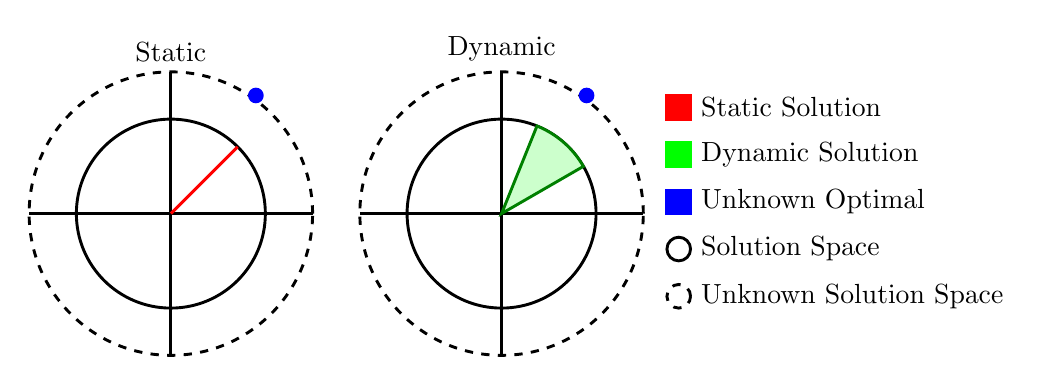
\begin{tikzpicture}[scale=0.6, line width=1.05][]

	\node at (0.0 , 1) [above] {Static};
    \draw (-3.0,  -2.0) -- ( 3.0,  -2.0);
	\draw ( 0.0, -5.0) -- ( 0.0,  1.0);
	\draw ( 0.0,  -2.0) circle [radius=2cm];
	\draw[dashed] ( 0.0,  -2.0) circle [radius=3.0cm];
	\node[blue] at (1.8, 0.5) [circle, fill, inner sep=2pt]{};
	\draw[red] (0.0, -2.0) -- ++(45:2.0);

	\node at (7.0 , 1) [above] {Dynamic};
    \draw ( 4.0,  -2.0) -- (10.0, -2.0);
	\draw ( 7.0, -5.0) -- ( 7.0, 1.0);
	\draw ( 7.0,  -2.0) circle [radius=2cm];
	\draw[dashed] ( 7.0,  -2.0) circle [radius=3.0cm];
	\node[blue] at (8.8, 0.5) [circle, fill, inner sep=2pt]{};
	\filldraw[fill=green!20,draw=green!50!black] (7,-2) -- ++(30:2.cm)
	        arc [start angle=30, end angle=68, radius=2.cm] -- cycle;
	
	\begin{scope}[shift={(10.5,0.5)}]
		% \node at (-0.25,1) [right] {};
		\draw[color=red,fill] (0,0.0)  rectangle  (0.5, -0.5);
		\node[anchor=west] at (0.5, -0.25) { Static Solution };

		\draw[color=green,fill] (0,-1.0)  rectangle  (0.5, -1.5);
		\node[anchor=west] at (0.5, -1.25) { Dynamic Solution };

		\draw[color=blue,fill] (0,-2.0)  rectangle  (0.5, -2.5);
		\node[anchor=west] at (0.5, -2.25) { Unknown Optimal };

		\draw[color=black] (0.25,-3.25)  circle  (0.25);
		\node[anchor=west] at (0.5, -3.25) { Solution Space };

		\draw[color=black,dashed] (0.25,-4.25)  circle  (0.25);
		\node[anchor=west] at (0.5, -4.25) { Unknown Solution Space };
	\end{scope}
    % \shade[ball color=red!50!white,opacity=0.8] (0,0) -- (90:\radius) arc (90:-90:\height) -- cycle;
	\end{tikzpicture}
}


			\drawReactiveConstraints{}

		\begin{itemize}
			\item Mathematical models guide direction but does not provide direct solutions.
			\item Static solutions are rarely fully executable.
			\item Dynamic models are less constrained and ensure a contained optimal solution.
			\item Remember: The real optimal solution is ever knowable at time = 0
		\end{itemize}
    \end{block}
\end{frame}

\begin{frame}[t]{}
    \begin{block}{}

		% \usetikzlibrary {positioning}
\definecolor{red}{HTML}{8A3F3A}
\definecolor{yellow}{HTML}{E0BB3C}
\definecolor{blue}{HTML}{4569E0}
\definecolor{green}{HTML}{17E561}
\definecolor{other}{HTML}{6A939E}

% DTU Colors
\definecolor{dtu-corporate-red}{HTML}{990000}
\definecolor{dtu-white}{HTML}{ffffff}
\definecolor{dtu-black}{HTML}{000000}
\definecolor{dtu-blue}{HTML}{2F3EEA}
\definecolor{dtu-bright-green}{HTML}{1FD082}
\definecolor{dtu-navy-blue}{HTML}{030F4F}
\definecolor{dtu-yellow}{HTML}{F6D04D}
\definecolor{dtu-orange}{HTML}{FC7634}
\definecolor{dtu-pink}{HTML}{F7BBB1}
\definecolor{dtu-grey}{HTML}{DADADA}
\definecolor{dtu-red}{HTML}{E83F48}
\definecolor{dtu-green}{HTML}{008835}
\definecolor{dtu-purple}{HTML}{79238E}




\newcommand{\drawHexagon}[4]{
	\draw[fill=#3] (#1,#2) ++(30:2) -- ++(90:2) -- ++(150:2) -- ++(210:2) -- ++(270:2) -- ++(330:2) -- ++(30:2);
	\node at (#1,#2) {#4};
}

\newcommand{\drawUncertaintyComplexityValue}{
	\begin{tikzpicture}[scale=0.6, line width=1.05][]

	% We should parameterize this! I think that is the best approach!
	\drawHexagon{2}{2}{dtu-red}{Strategic}
	\drawHexagon{{6 - 2 * (2 - sqrt(3)) }}{ 2}{dtu-red}{Strategic}
	\drawHexagon{{4 - 1 * (2 - sqrt(3)) }}{-1}{dtu-red}{Strategic}

	\drawHexagon{{0 + 1 * (2 - sqrt(3)) }}{-1}{dtu-red}{Strategic}
	\drawHexagon{{8 - 3 * (2 - sqrt(3)) }}{-1}{dtu-red}{Strategic}

	% \node at (0.0 , 1) [above] {Static};
    % \draw (-3.0,  -2.0) -- ( 3.0,  -2.0);
	% \draw ( 0.0, -5.0) -- ( 0.0,  1.0);
	% \draw ( 0.0,  -2.0) circle [radius=2cm];
	% \draw[dashed] ( 0.0,  -2.0) circle [radius=3.0cm];
	% \node[blue] at (1.8, 0.5) [circle, fill, inner sep=2pt]{};
	% \draw[red] (0.0, -2.0) -- ++(45:2.0);

	% \node at (7.0 , 1) [above] {Dynamic};
    % \draw ( 4.0,  -2.0) -- (10.0, -2.0);
	% \draw ( 7.0, -5.0) -- ( 7.0, 1.0);
	% \draw ( 7.0,  -2.0) circle [radius=2cm];
	% \draw[dashed] ( 7.0,  -2.0) circle [radius=3.0cm];
	% \node[blue] at (8.8, 0.5) [circle, fill, inner sep=2pt]{};
	% \filldraw[fill=green!20,draw=green!50!black] (7,-2) -- ++(30:2.cm)
	%         arc [start angle=30, end angle=68, radius=2.cm] -- cycle;

	
	% \begin{scope}[shift={(10.5,0.5)}]
	% 	% \node at (-0.25,1) [right] {};
	% 	\draw[color=red,fill] (0,0.0)  rectangle  (0.5, -0.5);
	% 	\node[anchor=west] at (0.5, -0.25) { Static Solution };

	% 	\draw[color=green,fill] (0,-1.0)  rectangle  (0.5, -1.5);
	% 	\node[anchor=west] at (0.5, -1.25) { Dynamic Solution };

	% 	\draw[color=blue,fill] (0,-2.0)  rectangle  (0.5, -2.5);
	% 	\node[anchor=west] at (0.5, -2.25) { Unknown Optimal };

	% 	\draw[color=black] (0.25,-3.25)  circle  (0.25);
	% 	\node[anchor=west] at (0.5, -3.25) { Solution Space };

	% 	\draw[color=black,dashed] (0.25,-4.25)  circle  (0.25);
	% 	\node[anchor=west] at (0.5, -4.25) { Unknown Solution Space };

		
	% \end{scope}

    % \shade[ball color=red!50!white,opacity=0.8] (0,0) -- (90:\radius) arc (90:-90:\height) -- cycle;

	\end{tikzpicture}
}



		% \drawUncertaintyComplexityValue[
		% 	show_useless_operation_research =true,			
		% 	show_simplistic_heuristics=true,
		% ]
		% \only<1>{}
		% \only<2>{

		% 	\begin{itemize}
		% 		\item An engineering trade off will have to be made
		% 	\end{itemize}
		% }


		
    \end{block}
\end{frame}

\begin{frame}[t]{}
    \begin{block}{Model setup}
		\usetikzlibrary {positioning}
\newcommand{\drawHexagon}[6][draw=black]{
	\draw[#1, fill=#4] (#2,#3) ++(30:#6) -- ++(90:#6) -- ++(150:#6) -- ++(210:#6) -- ++(270:#6) -- ++(330:#6) -- cycle;
	\node[align=center] at (#2,#3+2) {#5};
}

\newif\ifpersistencelayer
\newif\ifatomicpointerswaplayer
\newif\ifmetaheuristicslayer
\newif\ifuserinterfacelayer
\newif\iforchestratorlayer
\newif\ifsimplifiedlayer

\pgfkeys{
	/hexagon/.is family, /hexagon,
	default/.style = {
		persistence=false,
		atomicpointerswap=false,
		metaheuristics=false,
		orchestrator=false,
		userinterface=false,
		simplified=false,
	},
	persistence/.is if=persistencelayer,
	atomicpointerswap/.is if=atomicpointerswaplayer,
	metaheuristics/.is if=metaheuristicslayer,
	orchestrator/.is if=orchestratorlayer,
	userinterface/.is if=userinterfacelayer,
	simplified/.is if=simplifiedlayer,
}
\newcommand{\drawModelSetupHexagon}[1][]{
	\pgfkeys{/hexagon, default, #1}

	\begin{tikzpicture}[font=\footnotesize, scale=0.5, line width=1.05]
	

	\ifpersistencelayer
		\drawHexagon[draw=none]{ 2                      }{ 2}{dtu-blue}{}{2}
		\drawHexagon[draw=none]{{6 - 2 * (2 - sqrt(3)) }}{ 2}{dtu-blue}{}{2}
		\drawHexagon[draw=none]{{4 - 1 * (2 - sqrt(3)) }}{-1}{dtu-blue}{Persistence}{2}
		\drawHexagon[draw=none]{{0 + 1 * (2 - sqrt(3)) }}{-1}{dtu-blue}{}{2}
		\drawHexagon[draw=none]{{8 - 3 * (2 - sqrt(3)) }}{-1}{dtu-blue}{}{2}

		\drawHexagon[draw=none]{{2 - 0 * (2 - sqrt(3)) }}{-4}{dtu-blue}{}{2}
		\drawHexagon[draw=none]{{6 - 2 * (2 - sqrt(3)) }}{-4}{dtu-blue}{}{2}

		\drawHexagon[draw=none]{{10 - 4 * (2 - sqrt(3)) }}{-4}{dtu-blue}{}{2}
		\drawHexagon[draw=none]{{-2 + 2 * (2 - sqrt(3)) }}{-4}{dtu-blue}{}{2}

		\drawHexagon[draw=none]{{12 - 5 * (2 - sqrt(3)) }}{-1}{dtu-blue}{}{2}
		\drawHexagon[draw=none]{{-4 + 3 * (2 - sqrt(3)) }}{-1}{dtu-blue}{}{2}
		% Legend for each layer
		\drawHexagon{{14.0  }}{+3.0}{dtu-blue}{}{0.75}
		\node[align=right, anchor=west] at ({15.0}, +3.75) {Persistence};
		\drawHexagon{{14.0  }}{+1.5}{dtu-white}{}{0.75}
		\node[align=right, anchor=west] at ({15.0}, +2.25) {Atomic Pointer};
		\drawHexagon{{14.0  }}{+0.0}{dtu-white}{}{0.75}
		\node[align=right, anchor=west] at ({15.0}, +0.75) {Metaheuristics};
		\drawHexagon{{14.0  }}{-1.5}{dtu-white}{}{0.75}
		\node[align=right, anchor=west] at ({15.0}, -0.75) {Orchestration};
		\drawHexagon{{14.0  }}{-3.0}{dtu-white}{}{0.75}
		\node[align=right, anchor=west] at ({15.0}, -2.25) {User interfaces};
	\fi


	\ifatomicpointerswaplayer
		\drawHexagon[]{ 2                      }{ 2}{dtu-green}{Shared\\solution\\pointer}{2}
		\drawHexagon[]{{6 - 2 * (2 - sqrt(3)) }}{ 2}{dtu-green}{Shared\\solution\\pointer}{2}
		\drawHexagon[]{{4 - 1 * (2 - sqrt(3)) }}{-1}{dtu-green}{Shared\\solution\\pointer}{2}
		\drawHexagon[]{{0 + 1 * (2 - sqrt(3)) }}{-1}{dtu-green}{Shared\\solution\\pointer}{2}
		\drawHexagon[]{{8 - 3 * (2 - sqrt(3)) }}{-1}{dtu-green}{Shared\\solution\\pointer}{2}

		\drawHexagon[]{{2 - 0 * (2 - sqrt(3)) }}{-4}{dtu-green}{Shared\\solution\\pointer}{2}
		\drawHexagon[]{{6 - 2 * (2 - sqrt(3)) }}{-4}{dtu-green}{Shared\\solution\\pointer}{2}

		\drawHexagon[]{{10 - 4 * (2 - sqrt(3)) }}{-4}{dtu-green}{Shared\\solution\\pointer}{2}
		\drawHexagon[]{{-2 + 2 * (2 - sqrt(3)) }}{-4}{dtu-green}{Shared\\solution\\pointer}{2}

		\drawHexagon[]{{12 - 5 * (2 - sqrt(3)) }}{-1}{dtu-green}{Shared\\solution\\pointer}{2}
		\drawHexagon[]{{-4 + 3 * (2 - sqrt(3)) }}{-1}{dtu-green}{Shared\\solution\\pointer}{2}
		% Legend for each layer
		\drawHexagon{{14.0  }}{+3.0}{dtu-white}{}{0.75}
		\node[align=right, anchor=west] at ({15.0}, +3.75) {Persistence};
		\drawHexagon{{14.0  }}{+1.5}{dtu-green}{}{0.75}
		\node[align=right, anchor=west] at ({15.0}, +2.25) {Atomic Pointer};
		\drawHexagon{{14.0  }}{+0.0}{dtu-white}{}{0.75}
		\node[align=right, anchor=west] at ({15.0}, +0.75) {Metaheuristics};
		\drawHexagon{{14.0  }}{-1.5}{dtu-white}{}{0.75}
		\node[align=right, anchor=west] at ({15.0}, -0.75) {Orchestration};
		\drawHexagon{{14.0  }}{-3.0}{dtu-white}{}{0.75}
		\node[align=right, anchor=west] at ({15.0}, -2.25) {User interfaces};
	\fi

	\ifsimplifiedlayer

		\node[align=right, anchor=west] at ({-5.5}, +3.75) {};
		\drawHexagon{{+2 + 0 * (2 - sqrt(3)) }}{ 2}{dtu-green}{Scheduler}{2}
		\drawHexagon{{+4 - 1 * (2 - sqrt(3)) }}{-1}{dtu-red}{Supervisor}{2}
		\drawHexagon{{+0 + 1 * (2 - sqrt(3)) }}{-1}{dtu-red}{Supervisor}{2}
		\drawHexagon{{+2 - 0 * (2 - sqrt(3)) }}{-4}{dtu-corporate-red}{Technician}{2}
		\drawHexagon{{+6 - 2 * (2 - sqrt(3)) }}{-4}{dtu-corporate-red}{Technician}{2}
		\drawHexagon{{-2 + 2 * (2 - sqrt(3)) }}{-4}{dtu-corporate-red}{Technician}{2}
		\drawHexagon{{+8 - 3 * (2 - sqrt(3)) }}{-1}{dtu-corporate-red}{Technician}{2}
		\drawHexagon{{-4 + 3 * (2 - sqrt(3)) }}{-1}{dtu-corporate-red}{Technician}{2}

		% Scheduler
		\draw[thin, fill=dtu-yellow] (2, 5) circle (0.35);
		\draw[thin, fill=dtu-purple] (2, 3) circle (0.35);
		% Supervisor 1
		\draw[thin, fill=dtu-yellow] ({+4 - 1 * (2 - sqrt(3)) }, 02) circle (0.35);
		\draw[thin, fill=dtu-purple] ({+4 - 1 * (2 - sqrt(3)) }, -0) circle (0.35);
		% Supervisor 2
		\draw[thin, fill=dtu-yellow] ({+0 + 1 * (2 - sqrt(3)) }, 02) circle (0.35);
		\draw[thin, fill=dtu-purple] ({+0 + 1 * (2 - sqrt(3)) }, -0) circle (0.35);
		% Technician 1
		\draw[thin, fill=dtu-yellow] ({+2 - 0 * (2 - sqrt(3)) }, -1) circle (0.35);
		\draw[thin, fill=dtu-purple] ({+2 - 0 * (2 - sqrt(3)) }, -3) circle (0.35);
		% Technician 2
		\draw[thin, fill=dtu-yellow] ({+6 - 2 * (2 - sqrt(3)) }, -1) circle (0.35);
		\draw[thin, fill=dtu-purple] ({+6 - 2 * (2 - sqrt(3)) }, -3) circle (0.35);
		% Technician 3
		\draw[thin, fill=dtu-yellow] ({-2 + 2 * (2 - sqrt(3)) }, -1) circle (0.35);
		\draw[thin, fill=dtu-purple] ({-2 + 2 * (2 - sqrt(3)) }, -3) circle (0.35);
		% Technician 4
		\draw[thin, fill=dtu-yellow] ({+8 - 3 * (2 - sqrt(3)) }, 02) circle (0.35);
		\draw[thin, fill=dtu-purple] ({+8 - 3 * (2 - sqrt(3)) }, -0) circle (0.35);
		% Technician 5
		\draw[thin, fill=dtu-yellow] ({-4 + 3 * (2 - sqrt(3)) }, 02) circle (0.35);
		\draw[thin, fill=dtu-purple] ({-4 + 3 * (2 - sqrt(3)) }, -0) circle (0.35);

		% Legend for each layer
		\node[align=right, anchor=west] at ({12.0}, +3.75) {Atomic Pointer};
		\draw[fill=dtu-purple] (11.0,  +3.75) circle (0.5);

		\node[align=right, anchor=west] at ({12.0}, +2.25) {Scheduler Metaheuristic};
		\drawHexagon{{11.0  }}{+1.75}{dtu-green}{}{0.5}
		\node[align=right, anchor=west] at ({12.0}, +0.75) {Supervisor Metaheuristic};
		\drawHexagon{{11.0  }}{+0.25}{dtu-red}{}{0.5}
		\node[align=right, anchor=west] at ({12.0}, -0.75) {Technician Metaheuristic};
		\drawHexagon{{11.0  }}{-1.25}{dtu-corporate-red}{}{0.5}
		\node[align=right, anchor=west] at ({12.0}, -2.25) {User interfaces (Message Passing)};
		\draw[fill=dtu-yellow] (11.0, -2.25) circle (0.5);
	\fi

	\ifmetaheuristicslayer
		\drawHexagon{ 2                      }{ 2}{dtu-blue}{Strategic}{2}
		\drawHexagon{{6 - 2 * (2 - sqrt(3)) }}{ 2}{dtu-green}{Tactical}{2}
		\drawHexagon{{4 - 1 * (2 - sqrt(3)) }}{-1}{dtu-red}{Supervisor}{2}
		\drawHexagon{{0 + 1 * (2 - sqrt(3)) }}{-1}{dtu-red}{Supervisor}{2}
		\drawHexagon{{8 - 3 * (2 - sqrt(3)) }}{-1}{dtu-red}{Supervisor}{2}

		\drawHexagon{{2 - 0 * (2 - sqrt(3)) }}{-4}{dtu-corporate-red}{Technician}{2}
		\drawHexagon{{6 - 2 * (2 - sqrt(3)) }}{-4}{dtu-corporate-red}{Technician}{2}

		\drawHexagon{{10 - 4 * (2 - sqrt(3)) }}{-4}{dtu-corporate-red}{Technician}{2}
		\drawHexagon{{-2 + 2 * (2 - sqrt(3)) }}{-4}{dtu-corporate-red}{Technician}{2}

		\drawHexagon{{12 - 5 * (2 - sqrt(3)) }}{-1}{dtu-corporate-red}{Technician}{2}
		\drawHexagon{{-4 + 3 * (2 - sqrt(3)) }}{-1}{dtu-corporate-red}{Technician}{2}

		% Legend for each layer
		\drawHexagon{{14.0  }}{+3.0}{dtu-white}{}{0.75}
		\node[align=right, anchor=west] at ({15.0}, +3.75) {Persistence};
		\drawHexagon{{14.0  }}{+1.5}{dtu-white}{}{0.75}
		\node[align=right, anchor=west] at ({15.0}, +2.25) {Atomic Pointer};
		\drawHexagon{{14.0  }}{+0.0}{dtu-corporate-red}{}{0.75}
		\node[align=right, anchor=west] at ({15.0}, +0.75) {Metaheuristics};
		\drawHexagon{{14.0  }}{-1.5}{dtu-white}{}{0.75}
		\node[align=right, anchor=west] at ({15.0}, -0.75) {Orchestration};
		\drawHexagon{{14.0  }}{-3.0}{dtu-white}{}{0.75}
		\node[align=right, anchor=west] at ({15.0}, -2.25) {User interfaces};
	\fi

	\iforchestratorlayer
		\drawHexagon{ 2                      }{ 2}{dtu-orange}{}{2}
		\drawHexagon{{6 - 2 * (2 - sqrt(3)) }}{ 2}{dtu-orange}{}{2}
		\drawHexagon{{4 - 1 * (2 - sqrt(3)) }}{-1}{dtu-orange}{Orche-\\strator}{2}
		\drawHexagon{{0 + 1 * (2 - sqrt(3)) }}{-1}{dtu-orange}{}{2}
		\drawHexagon{{8 - 3 * (2 - sqrt(3)) }}{-1}{dtu-orange}{}{2}

		\drawHexagon{{2 - 0 * (2 - sqrt(3)) }}{-4}{dtu-orange}{}{2}
		\drawHexagon{{6 - 2 * (2 - sqrt(3)) }}{-4}{dtu-orange}{}{2}

		\drawHexagon{{10 - 4 * (2 - sqrt(3)) }}{-4}{dtu-orange}{}{2}
		\drawHexagon{{-2 + 2 * (2 - sqrt(3)) }}{-4}{dtu-orange}{}{2}

		\drawHexagon{{12 - 5 * (2 - sqrt(3)) }}{-1}{dtu-orange}{}{2}
		\drawHexagon{{-4 + 3 * (2 - sqrt(3)) }}{-1}{dtu-orange}{}{2}
		% Legend for each layer
		\drawHexagon{{14.0  }}{+3.0}{dtu-white}{}{0.75}
		\node[align=right, anchor=west] at ({15.0}, +3.75) {Persistence};
		\drawHexagon{{14.0  }}{+1.5}{dtu-white}{}{0.75}
		\node[align=right, anchor=west] at ({15.0}, +2.25) {Atomic Pointer};
		\drawHexagon{{14.0  }}{+0.0}{dtu-white}{}{0.75}
		\node[align=right, anchor=west] at ({15.0}, +0.75) {Metaheuristics};
		\drawHexagon{{14.0  }}{-1.5}{dtu-orange}{}{0.75}
		\node[align=right, anchor=west] at ({15.0}, -0.75) {Orchestration};
		\drawHexagon{{14.0  }}{-3.0}{dtu-white}{}{0.75}
		\node[align=right, anchor=west] at ({15.0}, -2.25) {User interfaces};
	\fi

	
	\ifuserinterfacelayer
		\drawHexagon{ 2                      }{ 2}{dtu-yellow}{UI}{2}
		\drawHexagon{{6 - 2 * (2 - sqrt(3)) }}{ 2}{dtu-yellow}{UI}{2}
		\drawHexagon{{4 - 1 * (2 - sqrt(3)) }}{-1}{dtu-yellow}{UI}{2}
		\drawHexagon{{0 + 1 * (2 - sqrt(3)) }}{-1}{dtu-yellow}{UI}{2}
		\drawHexagon{{8 - 3 * (2 - sqrt(3)) }}{-1}{dtu-yellow}{UI}{2}

		\drawHexagon{{2 - 0 * (2 - sqrt(3)) }}{-4}{dtu-yellow}{UI}{2}
		\drawHexagon{{6 - 2 * (2 - sqrt(3)) }}{-4}{dtu-yellow}{UI}{2}

		\drawHexagon{{10 - 4 * (2 - sqrt(3)) }}{-4}{dtu-yellow}{UI}{2}
		\drawHexagon{{-2 + 2 * (2 - sqrt(3)) }}{-4}{dtu-yellow}{UI}{2}

		\drawHexagon{{12 - 5 * (2 - sqrt(3)) }}{-1}{dtu-yellow}{UI}{2}
		\drawHexagon{{-4 + 3 * (2 - sqrt(3)) }}{-1}{dtu-yellow}{UI}{2}
		% Legend for each layer
		\drawHexagon{{14.0  }}{+3.0}{dtu-white}{}{0.75}
		\node[align=right, anchor=west] at ({15.0}, +3.75) {Persistence};
		\drawHexagon{{14.0  }}{+1.5}{dtu-white}{}{0.75}
		\node[align=right, anchor=west] at ({15.0}, +2.25) {Atomic Pointer};
		\drawHexagon{{14.0  }}{+0.0}{dtu-white}{}{0.75}
		\node[align=right, anchor=west] at ({15.0}, +0.75) {Metaheuristics};
		\drawHexagon{{14.0  }}{-1.5}{dtu-white}{}{0.75}
		\node[align=right, anchor=west] at ({15.0}, -0.75) {Orchestration};
		\drawHexagon{{14.0  }}{-3.0}{dtu-yellow}{}{0.75}
		\node[align=right, anchor=west] at ({15.0}, -2.25) {User interfaces};
	\fi
	
	\end{tikzpicture}
}

		\drawModelSetupHexagon[persistence=true]
    \end{block}
\end{frame}

\begin{frame}[t]{}
    \begin{block}{Model setup}
		\usetikzlibrary {positioning}
\newcommand{\drawHexagon}[6][draw=black]{
	\draw[#1, fill=#4] (#2,#3) ++(30:#6) -- ++(90:#6) -- ++(150:#6) -- ++(210:#6) -- ++(270:#6) -- ++(330:#6) -- cycle;
	\node[align=center] at (#2,#3+2) {#5};
}

\newif\ifpersistencelayer
\newif\ifatomicpointerswaplayer
\newif\ifmetaheuristicslayer
\newif\ifuserinterfacelayer
\newif\iforchestratorlayer
\newif\ifsimplifiedlayer

\pgfkeys{
	/hexagon/.is family, /hexagon,
	default/.style = {
		persistence=false,
		atomicpointerswap=false,
		metaheuristics=false,
		orchestrator=false,
		userinterface=false,
		simplified=false,
	},
	persistence/.is if=persistencelayer,
	atomicpointerswap/.is if=atomicpointerswaplayer,
	metaheuristics/.is if=metaheuristicslayer,
	orchestrator/.is if=orchestratorlayer,
	userinterface/.is if=userinterfacelayer,
	simplified/.is if=simplifiedlayer,
}
\newcommand{\drawModelSetupHexagon}[1][]{
	\pgfkeys{/hexagon, default, #1}

	\begin{tikzpicture}[font=\footnotesize, scale=0.5, line width=1.05]
	

	\ifpersistencelayer
		\drawHexagon[draw=none]{ 2                      }{ 2}{dtu-blue}{}{2}
		\drawHexagon[draw=none]{{6 - 2 * (2 - sqrt(3)) }}{ 2}{dtu-blue}{}{2}
		\drawHexagon[draw=none]{{4 - 1 * (2 - sqrt(3)) }}{-1}{dtu-blue}{Persistence}{2}
		\drawHexagon[draw=none]{{0 + 1 * (2 - sqrt(3)) }}{-1}{dtu-blue}{}{2}
		\drawHexagon[draw=none]{{8 - 3 * (2 - sqrt(3)) }}{-1}{dtu-blue}{}{2}

		\drawHexagon[draw=none]{{2 - 0 * (2 - sqrt(3)) }}{-4}{dtu-blue}{}{2}
		\drawHexagon[draw=none]{{6 - 2 * (2 - sqrt(3)) }}{-4}{dtu-blue}{}{2}

		\drawHexagon[draw=none]{{10 - 4 * (2 - sqrt(3)) }}{-4}{dtu-blue}{}{2}
		\drawHexagon[draw=none]{{-2 + 2 * (2 - sqrt(3)) }}{-4}{dtu-blue}{}{2}

		\drawHexagon[draw=none]{{12 - 5 * (2 - sqrt(3)) }}{-1}{dtu-blue}{}{2}
		\drawHexagon[draw=none]{{-4 + 3 * (2 - sqrt(3)) }}{-1}{dtu-blue}{}{2}
		% Legend for each layer
		\drawHexagon{{14.0  }}{+3.0}{dtu-blue}{}{0.75}
		\node[align=right, anchor=west] at ({15.0}, +3.75) {Persistence};
		\drawHexagon{{14.0  }}{+1.5}{dtu-white}{}{0.75}
		\node[align=right, anchor=west] at ({15.0}, +2.25) {Atomic Pointer};
		\drawHexagon{{14.0  }}{+0.0}{dtu-white}{}{0.75}
		\node[align=right, anchor=west] at ({15.0}, +0.75) {Metaheuristics};
		\drawHexagon{{14.0  }}{-1.5}{dtu-white}{}{0.75}
		\node[align=right, anchor=west] at ({15.0}, -0.75) {Orchestration};
		\drawHexagon{{14.0  }}{-3.0}{dtu-white}{}{0.75}
		\node[align=right, anchor=west] at ({15.0}, -2.25) {User interfaces};
	\fi


	\ifatomicpointerswaplayer
		\drawHexagon[]{ 2                      }{ 2}{dtu-green}{Shared\\solution\\pointer}{2}
		\drawHexagon[]{{6 - 2 * (2 - sqrt(3)) }}{ 2}{dtu-green}{Shared\\solution\\pointer}{2}
		\drawHexagon[]{{4 - 1 * (2 - sqrt(3)) }}{-1}{dtu-green}{Shared\\solution\\pointer}{2}
		\drawHexagon[]{{0 + 1 * (2 - sqrt(3)) }}{-1}{dtu-green}{Shared\\solution\\pointer}{2}
		\drawHexagon[]{{8 - 3 * (2 - sqrt(3)) }}{-1}{dtu-green}{Shared\\solution\\pointer}{2}

		\drawHexagon[]{{2 - 0 * (2 - sqrt(3)) }}{-4}{dtu-green}{Shared\\solution\\pointer}{2}
		\drawHexagon[]{{6 - 2 * (2 - sqrt(3)) }}{-4}{dtu-green}{Shared\\solution\\pointer}{2}

		\drawHexagon[]{{10 - 4 * (2 - sqrt(3)) }}{-4}{dtu-green}{Shared\\solution\\pointer}{2}
		\drawHexagon[]{{-2 + 2 * (2 - sqrt(3)) }}{-4}{dtu-green}{Shared\\solution\\pointer}{2}

		\drawHexagon[]{{12 - 5 * (2 - sqrt(3)) }}{-1}{dtu-green}{Shared\\solution\\pointer}{2}
		\drawHexagon[]{{-4 + 3 * (2 - sqrt(3)) }}{-1}{dtu-green}{Shared\\solution\\pointer}{2}
		% Legend for each layer
		\drawHexagon{{14.0  }}{+3.0}{dtu-white}{}{0.75}
		\node[align=right, anchor=west] at ({15.0}, +3.75) {Persistence};
		\drawHexagon{{14.0  }}{+1.5}{dtu-green}{}{0.75}
		\node[align=right, anchor=west] at ({15.0}, +2.25) {Atomic Pointer};
		\drawHexagon{{14.0  }}{+0.0}{dtu-white}{}{0.75}
		\node[align=right, anchor=west] at ({15.0}, +0.75) {Metaheuristics};
		\drawHexagon{{14.0  }}{-1.5}{dtu-white}{}{0.75}
		\node[align=right, anchor=west] at ({15.0}, -0.75) {Orchestration};
		\drawHexagon{{14.0  }}{-3.0}{dtu-white}{}{0.75}
		\node[align=right, anchor=west] at ({15.0}, -2.25) {User interfaces};
	\fi

	\ifsimplifiedlayer

		\node[align=right, anchor=west] at ({-5.5}, +3.75) {};
		\drawHexagon{{+2 + 0 * (2 - sqrt(3)) }}{ 2}{dtu-green}{Scheduler}{2}
		\drawHexagon{{+4 - 1 * (2 - sqrt(3)) }}{-1}{dtu-red}{Supervisor}{2}
		\drawHexagon{{+0 + 1 * (2 - sqrt(3)) }}{-1}{dtu-red}{Supervisor}{2}
		\drawHexagon{{+2 - 0 * (2 - sqrt(3)) }}{-4}{dtu-corporate-red}{Technician}{2}
		\drawHexagon{{+6 - 2 * (2 - sqrt(3)) }}{-4}{dtu-corporate-red}{Technician}{2}
		\drawHexagon{{-2 + 2 * (2 - sqrt(3)) }}{-4}{dtu-corporate-red}{Technician}{2}
		\drawHexagon{{+8 - 3 * (2 - sqrt(3)) }}{-1}{dtu-corporate-red}{Technician}{2}
		\drawHexagon{{-4 + 3 * (2 - sqrt(3)) }}{-1}{dtu-corporate-red}{Technician}{2}

		% Scheduler
		\draw[thin, fill=dtu-yellow] (2, 5) circle (0.35);
		\draw[thin, fill=dtu-purple] (2, 3) circle (0.35);
		% Supervisor 1
		\draw[thin, fill=dtu-yellow] ({+4 - 1 * (2 - sqrt(3)) }, 02) circle (0.35);
		\draw[thin, fill=dtu-purple] ({+4 - 1 * (2 - sqrt(3)) }, -0) circle (0.35);
		% Supervisor 2
		\draw[thin, fill=dtu-yellow] ({+0 + 1 * (2 - sqrt(3)) }, 02) circle (0.35);
		\draw[thin, fill=dtu-purple] ({+0 + 1 * (2 - sqrt(3)) }, -0) circle (0.35);
		% Technician 1
		\draw[thin, fill=dtu-yellow] ({+2 - 0 * (2 - sqrt(3)) }, -1) circle (0.35);
		\draw[thin, fill=dtu-purple] ({+2 - 0 * (2 - sqrt(3)) }, -3) circle (0.35);
		% Technician 2
		\draw[thin, fill=dtu-yellow] ({+6 - 2 * (2 - sqrt(3)) }, -1) circle (0.35);
		\draw[thin, fill=dtu-purple] ({+6 - 2 * (2 - sqrt(3)) }, -3) circle (0.35);
		% Technician 3
		\draw[thin, fill=dtu-yellow] ({-2 + 2 * (2 - sqrt(3)) }, -1) circle (0.35);
		\draw[thin, fill=dtu-purple] ({-2 + 2 * (2 - sqrt(3)) }, -3) circle (0.35);
		% Technician 4
		\draw[thin, fill=dtu-yellow] ({+8 - 3 * (2 - sqrt(3)) }, 02) circle (0.35);
		\draw[thin, fill=dtu-purple] ({+8 - 3 * (2 - sqrt(3)) }, -0) circle (0.35);
		% Technician 5
		\draw[thin, fill=dtu-yellow] ({-4 + 3 * (2 - sqrt(3)) }, 02) circle (0.35);
		\draw[thin, fill=dtu-purple] ({-4 + 3 * (2 - sqrt(3)) }, -0) circle (0.35);

		% Legend for each layer
		\node[align=right, anchor=west] at ({12.0}, +3.75) {Atomic Pointer};
		\draw[fill=dtu-purple] (11.0,  +3.75) circle (0.5);

		\node[align=right, anchor=west] at ({12.0}, +2.25) {Scheduler Metaheuristic};
		\drawHexagon{{11.0  }}{+1.75}{dtu-green}{}{0.5}
		\node[align=right, anchor=west] at ({12.0}, +0.75) {Supervisor Metaheuristic};
		\drawHexagon{{11.0  }}{+0.25}{dtu-red}{}{0.5}
		\node[align=right, anchor=west] at ({12.0}, -0.75) {Technician Metaheuristic};
		\drawHexagon{{11.0  }}{-1.25}{dtu-corporate-red}{}{0.5}
		\node[align=right, anchor=west] at ({12.0}, -2.25) {User interfaces (Message Passing)};
		\draw[fill=dtu-yellow] (11.0, -2.25) circle (0.5);
	\fi

	\ifmetaheuristicslayer
		\drawHexagon{ 2                      }{ 2}{dtu-blue}{Strategic}{2}
		\drawHexagon{{6 - 2 * (2 - sqrt(3)) }}{ 2}{dtu-green}{Tactical}{2}
		\drawHexagon{{4 - 1 * (2 - sqrt(3)) }}{-1}{dtu-red}{Supervisor}{2}
		\drawHexagon{{0 + 1 * (2 - sqrt(3)) }}{-1}{dtu-red}{Supervisor}{2}
		\drawHexagon{{8 - 3 * (2 - sqrt(3)) }}{-1}{dtu-red}{Supervisor}{2}

		\drawHexagon{{2 - 0 * (2 - sqrt(3)) }}{-4}{dtu-corporate-red}{Technician}{2}
		\drawHexagon{{6 - 2 * (2 - sqrt(3)) }}{-4}{dtu-corporate-red}{Technician}{2}

		\drawHexagon{{10 - 4 * (2 - sqrt(3)) }}{-4}{dtu-corporate-red}{Technician}{2}
		\drawHexagon{{-2 + 2 * (2 - sqrt(3)) }}{-4}{dtu-corporate-red}{Technician}{2}

		\drawHexagon{{12 - 5 * (2 - sqrt(3)) }}{-1}{dtu-corporate-red}{Technician}{2}
		\drawHexagon{{-4 + 3 * (2 - sqrt(3)) }}{-1}{dtu-corporate-red}{Technician}{2}

		% Legend for each layer
		\drawHexagon{{14.0  }}{+3.0}{dtu-white}{}{0.75}
		\node[align=right, anchor=west] at ({15.0}, +3.75) {Persistence};
		\drawHexagon{{14.0  }}{+1.5}{dtu-white}{}{0.75}
		\node[align=right, anchor=west] at ({15.0}, +2.25) {Atomic Pointer};
		\drawHexagon{{14.0  }}{+0.0}{dtu-corporate-red}{}{0.75}
		\node[align=right, anchor=west] at ({15.0}, +0.75) {Metaheuristics};
		\drawHexagon{{14.0  }}{-1.5}{dtu-white}{}{0.75}
		\node[align=right, anchor=west] at ({15.0}, -0.75) {Orchestration};
		\drawHexagon{{14.0  }}{-3.0}{dtu-white}{}{0.75}
		\node[align=right, anchor=west] at ({15.0}, -2.25) {User interfaces};
	\fi

	\iforchestratorlayer
		\drawHexagon{ 2                      }{ 2}{dtu-orange}{}{2}
		\drawHexagon{{6 - 2 * (2 - sqrt(3)) }}{ 2}{dtu-orange}{}{2}
		\drawHexagon{{4 - 1 * (2 - sqrt(3)) }}{-1}{dtu-orange}{Orche-\\strator}{2}
		\drawHexagon{{0 + 1 * (2 - sqrt(3)) }}{-1}{dtu-orange}{}{2}
		\drawHexagon{{8 - 3 * (2 - sqrt(3)) }}{-1}{dtu-orange}{}{2}

		\drawHexagon{{2 - 0 * (2 - sqrt(3)) }}{-4}{dtu-orange}{}{2}
		\drawHexagon{{6 - 2 * (2 - sqrt(3)) }}{-4}{dtu-orange}{}{2}

		\drawHexagon{{10 - 4 * (2 - sqrt(3)) }}{-4}{dtu-orange}{}{2}
		\drawHexagon{{-2 + 2 * (2 - sqrt(3)) }}{-4}{dtu-orange}{}{2}

		\drawHexagon{{12 - 5 * (2 - sqrt(3)) }}{-1}{dtu-orange}{}{2}
		\drawHexagon{{-4 + 3 * (2 - sqrt(3)) }}{-1}{dtu-orange}{}{2}
		% Legend for each layer
		\drawHexagon{{14.0  }}{+3.0}{dtu-white}{}{0.75}
		\node[align=right, anchor=west] at ({15.0}, +3.75) {Persistence};
		\drawHexagon{{14.0  }}{+1.5}{dtu-white}{}{0.75}
		\node[align=right, anchor=west] at ({15.0}, +2.25) {Atomic Pointer};
		\drawHexagon{{14.0  }}{+0.0}{dtu-white}{}{0.75}
		\node[align=right, anchor=west] at ({15.0}, +0.75) {Metaheuristics};
		\drawHexagon{{14.0  }}{-1.5}{dtu-orange}{}{0.75}
		\node[align=right, anchor=west] at ({15.0}, -0.75) {Orchestration};
		\drawHexagon{{14.0  }}{-3.0}{dtu-white}{}{0.75}
		\node[align=right, anchor=west] at ({15.0}, -2.25) {User interfaces};
	\fi

	
	\ifuserinterfacelayer
		\drawHexagon{ 2                      }{ 2}{dtu-yellow}{UI}{2}
		\drawHexagon{{6 - 2 * (2 - sqrt(3)) }}{ 2}{dtu-yellow}{UI}{2}
		\drawHexagon{{4 - 1 * (2 - sqrt(3)) }}{-1}{dtu-yellow}{UI}{2}
		\drawHexagon{{0 + 1 * (2 - sqrt(3)) }}{-1}{dtu-yellow}{UI}{2}
		\drawHexagon{{8 - 3 * (2 - sqrt(3)) }}{-1}{dtu-yellow}{UI}{2}

		\drawHexagon{{2 - 0 * (2 - sqrt(3)) }}{-4}{dtu-yellow}{UI}{2}
		\drawHexagon{{6 - 2 * (2 - sqrt(3)) }}{-4}{dtu-yellow}{UI}{2}

		\drawHexagon{{10 - 4 * (2 - sqrt(3)) }}{-4}{dtu-yellow}{UI}{2}
		\drawHexagon{{-2 + 2 * (2 - sqrt(3)) }}{-4}{dtu-yellow}{UI}{2}

		\drawHexagon{{12 - 5 * (2 - sqrt(3)) }}{-1}{dtu-yellow}{UI}{2}
		\drawHexagon{{-4 + 3 * (2 - sqrt(3)) }}{-1}{dtu-yellow}{UI}{2}
		% Legend for each layer
		\drawHexagon{{14.0  }}{+3.0}{dtu-white}{}{0.75}
		\node[align=right, anchor=west] at ({15.0}, +3.75) {Persistence};
		\drawHexagon{{14.0  }}{+1.5}{dtu-white}{}{0.75}
		\node[align=right, anchor=west] at ({15.0}, +2.25) {Atomic Pointer};
		\drawHexagon{{14.0  }}{+0.0}{dtu-white}{}{0.75}
		\node[align=right, anchor=west] at ({15.0}, +0.75) {Metaheuristics};
		\drawHexagon{{14.0  }}{-1.5}{dtu-white}{}{0.75}
		\node[align=right, anchor=west] at ({15.0}, -0.75) {Orchestration};
		\drawHexagon{{14.0  }}{-3.0}{dtu-yellow}{}{0.75}
		\node[align=right, anchor=west] at ({15.0}, -2.25) {User interfaces};
	\fi
	
	\end{tikzpicture}
}

		\drawModelSetupHexagon[atomicpointerswap=true]
    \end{block}
\end{frame}

\begin{frame}[t]{}
    \begin{block}{Model setup}
		\usetikzlibrary {positioning}
\newcommand{\drawHexagon}[6][draw=black]{
	\draw[#1, fill=#4] (#2,#3) ++(30:#6) -- ++(90:#6) -- ++(150:#6) -- ++(210:#6) -- ++(270:#6) -- ++(330:#6) -- cycle;
	\node[align=center] at (#2,#3+2) {#5};
}

\newif\ifpersistencelayer
\newif\ifatomicpointerswaplayer
\newif\ifmetaheuristicslayer
\newif\ifuserinterfacelayer
\newif\iforchestratorlayer
\newif\ifsimplifiedlayer

\pgfkeys{
	/hexagon/.is family, /hexagon,
	default/.style = {
		persistence=false,
		atomicpointerswap=false,
		metaheuristics=false,
		orchestrator=false,
		userinterface=false,
		simplified=false,
	},
	persistence/.is if=persistencelayer,
	atomicpointerswap/.is if=atomicpointerswaplayer,
	metaheuristics/.is if=metaheuristicslayer,
	orchestrator/.is if=orchestratorlayer,
	userinterface/.is if=userinterfacelayer,
	simplified/.is if=simplifiedlayer,
}
\newcommand{\drawModelSetupHexagon}[1][]{
	\pgfkeys{/hexagon, default, #1}

	\begin{tikzpicture}[font=\footnotesize, scale=0.5, line width=1.05]
	

	\ifpersistencelayer
		\drawHexagon[draw=none]{ 2                      }{ 2}{dtu-blue}{}{2}
		\drawHexagon[draw=none]{{6 - 2 * (2 - sqrt(3)) }}{ 2}{dtu-blue}{}{2}
		\drawHexagon[draw=none]{{4 - 1 * (2 - sqrt(3)) }}{-1}{dtu-blue}{Persistence}{2}
		\drawHexagon[draw=none]{{0 + 1 * (2 - sqrt(3)) }}{-1}{dtu-blue}{}{2}
		\drawHexagon[draw=none]{{8 - 3 * (2 - sqrt(3)) }}{-1}{dtu-blue}{}{2}

		\drawHexagon[draw=none]{{2 - 0 * (2 - sqrt(3)) }}{-4}{dtu-blue}{}{2}
		\drawHexagon[draw=none]{{6 - 2 * (2 - sqrt(3)) }}{-4}{dtu-blue}{}{2}

		\drawHexagon[draw=none]{{10 - 4 * (2 - sqrt(3)) }}{-4}{dtu-blue}{}{2}
		\drawHexagon[draw=none]{{-2 + 2 * (2 - sqrt(3)) }}{-4}{dtu-blue}{}{2}

		\drawHexagon[draw=none]{{12 - 5 * (2 - sqrt(3)) }}{-1}{dtu-blue}{}{2}
		\drawHexagon[draw=none]{{-4 + 3 * (2 - sqrt(3)) }}{-1}{dtu-blue}{}{2}
		% Legend for each layer
		\drawHexagon{{14.0  }}{+3.0}{dtu-blue}{}{0.75}
		\node[align=right, anchor=west] at ({15.0}, +3.75) {Persistence};
		\drawHexagon{{14.0  }}{+1.5}{dtu-white}{}{0.75}
		\node[align=right, anchor=west] at ({15.0}, +2.25) {Atomic Pointer};
		\drawHexagon{{14.0  }}{+0.0}{dtu-white}{}{0.75}
		\node[align=right, anchor=west] at ({15.0}, +0.75) {Metaheuristics};
		\drawHexagon{{14.0  }}{-1.5}{dtu-white}{}{0.75}
		\node[align=right, anchor=west] at ({15.0}, -0.75) {Orchestration};
		\drawHexagon{{14.0  }}{-3.0}{dtu-white}{}{0.75}
		\node[align=right, anchor=west] at ({15.0}, -2.25) {User interfaces};
	\fi


	\ifatomicpointerswaplayer
		\drawHexagon[]{ 2                      }{ 2}{dtu-green}{Shared\\solution\\pointer}{2}
		\drawHexagon[]{{6 - 2 * (2 - sqrt(3)) }}{ 2}{dtu-green}{Shared\\solution\\pointer}{2}
		\drawHexagon[]{{4 - 1 * (2 - sqrt(3)) }}{-1}{dtu-green}{Shared\\solution\\pointer}{2}
		\drawHexagon[]{{0 + 1 * (2 - sqrt(3)) }}{-1}{dtu-green}{Shared\\solution\\pointer}{2}
		\drawHexagon[]{{8 - 3 * (2 - sqrt(3)) }}{-1}{dtu-green}{Shared\\solution\\pointer}{2}

		\drawHexagon[]{{2 - 0 * (2 - sqrt(3)) }}{-4}{dtu-green}{Shared\\solution\\pointer}{2}
		\drawHexagon[]{{6 - 2 * (2 - sqrt(3)) }}{-4}{dtu-green}{Shared\\solution\\pointer}{2}

		\drawHexagon[]{{10 - 4 * (2 - sqrt(3)) }}{-4}{dtu-green}{Shared\\solution\\pointer}{2}
		\drawHexagon[]{{-2 + 2 * (2 - sqrt(3)) }}{-4}{dtu-green}{Shared\\solution\\pointer}{2}

		\drawHexagon[]{{12 - 5 * (2 - sqrt(3)) }}{-1}{dtu-green}{Shared\\solution\\pointer}{2}
		\drawHexagon[]{{-4 + 3 * (2 - sqrt(3)) }}{-1}{dtu-green}{Shared\\solution\\pointer}{2}
		% Legend for each layer
		\drawHexagon{{14.0  }}{+3.0}{dtu-white}{}{0.75}
		\node[align=right, anchor=west] at ({15.0}, +3.75) {Persistence};
		\drawHexagon{{14.0  }}{+1.5}{dtu-green}{}{0.75}
		\node[align=right, anchor=west] at ({15.0}, +2.25) {Atomic Pointer};
		\drawHexagon{{14.0  }}{+0.0}{dtu-white}{}{0.75}
		\node[align=right, anchor=west] at ({15.0}, +0.75) {Metaheuristics};
		\drawHexagon{{14.0  }}{-1.5}{dtu-white}{}{0.75}
		\node[align=right, anchor=west] at ({15.0}, -0.75) {Orchestration};
		\drawHexagon{{14.0  }}{-3.0}{dtu-white}{}{0.75}
		\node[align=right, anchor=west] at ({15.0}, -2.25) {User interfaces};
	\fi

	\ifsimplifiedlayer

		\node[align=right, anchor=west] at ({-5.5}, +3.75) {};
		\drawHexagon{{+2 + 0 * (2 - sqrt(3)) }}{ 2}{dtu-green}{Scheduler}{2}
		\drawHexagon{{+4 - 1 * (2 - sqrt(3)) }}{-1}{dtu-red}{Supervisor}{2}
		\drawHexagon{{+0 + 1 * (2 - sqrt(3)) }}{-1}{dtu-red}{Supervisor}{2}
		\drawHexagon{{+2 - 0 * (2 - sqrt(3)) }}{-4}{dtu-corporate-red}{Technician}{2}
		\drawHexagon{{+6 - 2 * (2 - sqrt(3)) }}{-4}{dtu-corporate-red}{Technician}{2}
		\drawHexagon{{-2 + 2 * (2 - sqrt(3)) }}{-4}{dtu-corporate-red}{Technician}{2}
		\drawHexagon{{+8 - 3 * (2 - sqrt(3)) }}{-1}{dtu-corporate-red}{Technician}{2}
		\drawHexagon{{-4 + 3 * (2 - sqrt(3)) }}{-1}{dtu-corporate-red}{Technician}{2}

		% Scheduler
		\draw[thin, fill=dtu-yellow] (2, 5) circle (0.35);
		\draw[thin, fill=dtu-purple] (2, 3) circle (0.35);
		% Supervisor 1
		\draw[thin, fill=dtu-yellow] ({+4 - 1 * (2 - sqrt(3)) }, 02) circle (0.35);
		\draw[thin, fill=dtu-purple] ({+4 - 1 * (2 - sqrt(3)) }, -0) circle (0.35);
		% Supervisor 2
		\draw[thin, fill=dtu-yellow] ({+0 + 1 * (2 - sqrt(3)) }, 02) circle (0.35);
		\draw[thin, fill=dtu-purple] ({+0 + 1 * (2 - sqrt(3)) }, -0) circle (0.35);
		% Technician 1
		\draw[thin, fill=dtu-yellow] ({+2 - 0 * (2 - sqrt(3)) }, -1) circle (0.35);
		\draw[thin, fill=dtu-purple] ({+2 - 0 * (2 - sqrt(3)) }, -3) circle (0.35);
		% Technician 2
		\draw[thin, fill=dtu-yellow] ({+6 - 2 * (2 - sqrt(3)) }, -1) circle (0.35);
		\draw[thin, fill=dtu-purple] ({+6 - 2 * (2 - sqrt(3)) }, -3) circle (0.35);
		% Technician 3
		\draw[thin, fill=dtu-yellow] ({-2 + 2 * (2 - sqrt(3)) }, -1) circle (0.35);
		\draw[thin, fill=dtu-purple] ({-2 + 2 * (2 - sqrt(3)) }, -3) circle (0.35);
		% Technician 4
		\draw[thin, fill=dtu-yellow] ({+8 - 3 * (2 - sqrt(3)) }, 02) circle (0.35);
		\draw[thin, fill=dtu-purple] ({+8 - 3 * (2 - sqrt(3)) }, -0) circle (0.35);
		% Technician 5
		\draw[thin, fill=dtu-yellow] ({-4 + 3 * (2 - sqrt(3)) }, 02) circle (0.35);
		\draw[thin, fill=dtu-purple] ({-4 + 3 * (2 - sqrt(3)) }, -0) circle (0.35);

		% Legend for each layer
		\node[align=right, anchor=west] at ({12.0}, +3.75) {Atomic Pointer};
		\draw[fill=dtu-purple] (11.0,  +3.75) circle (0.5);

		\node[align=right, anchor=west] at ({12.0}, +2.25) {Scheduler Metaheuristic};
		\drawHexagon{{11.0  }}{+1.75}{dtu-green}{}{0.5}
		\node[align=right, anchor=west] at ({12.0}, +0.75) {Supervisor Metaheuristic};
		\drawHexagon{{11.0  }}{+0.25}{dtu-red}{}{0.5}
		\node[align=right, anchor=west] at ({12.0}, -0.75) {Technician Metaheuristic};
		\drawHexagon{{11.0  }}{-1.25}{dtu-corporate-red}{}{0.5}
		\node[align=right, anchor=west] at ({12.0}, -2.25) {User interfaces (Message Passing)};
		\draw[fill=dtu-yellow] (11.0, -2.25) circle (0.5);
	\fi

	\ifmetaheuristicslayer
		\drawHexagon{ 2                      }{ 2}{dtu-blue}{Strategic}{2}
		\drawHexagon{{6 - 2 * (2 - sqrt(3)) }}{ 2}{dtu-green}{Tactical}{2}
		\drawHexagon{{4 - 1 * (2 - sqrt(3)) }}{-1}{dtu-red}{Supervisor}{2}
		\drawHexagon{{0 + 1 * (2 - sqrt(3)) }}{-1}{dtu-red}{Supervisor}{2}
		\drawHexagon{{8 - 3 * (2 - sqrt(3)) }}{-1}{dtu-red}{Supervisor}{2}

		\drawHexagon{{2 - 0 * (2 - sqrt(3)) }}{-4}{dtu-corporate-red}{Technician}{2}
		\drawHexagon{{6 - 2 * (2 - sqrt(3)) }}{-4}{dtu-corporate-red}{Technician}{2}

		\drawHexagon{{10 - 4 * (2 - sqrt(3)) }}{-4}{dtu-corporate-red}{Technician}{2}
		\drawHexagon{{-2 + 2 * (2 - sqrt(3)) }}{-4}{dtu-corporate-red}{Technician}{2}

		\drawHexagon{{12 - 5 * (2 - sqrt(3)) }}{-1}{dtu-corporate-red}{Technician}{2}
		\drawHexagon{{-4 + 3 * (2 - sqrt(3)) }}{-1}{dtu-corporate-red}{Technician}{2}

		% Legend for each layer
		\drawHexagon{{14.0  }}{+3.0}{dtu-white}{}{0.75}
		\node[align=right, anchor=west] at ({15.0}, +3.75) {Persistence};
		\drawHexagon{{14.0  }}{+1.5}{dtu-white}{}{0.75}
		\node[align=right, anchor=west] at ({15.0}, +2.25) {Atomic Pointer};
		\drawHexagon{{14.0  }}{+0.0}{dtu-corporate-red}{}{0.75}
		\node[align=right, anchor=west] at ({15.0}, +0.75) {Metaheuristics};
		\drawHexagon{{14.0  }}{-1.5}{dtu-white}{}{0.75}
		\node[align=right, anchor=west] at ({15.0}, -0.75) {Orchestration};
		\drawHexagon{{14.0  }}{-3.0}{dtu-white}{}{0.75}
		\node[align=right, anchor=west] at ({15.0}, -2.25) {User interfaces};
	\fi

	\iforchestratorlayer
		\drawHexagon{ 2                      }{ 2}{dtu-orange}{}{2}
		\drawHexagon{{6 - 2 * (2 - sqrt(3)) }}{ 2}{dtu-orange}{}{2}
		\drawHexagon{{4 - 1 * (2 - sqrt(3)) }}{-1}{dtu-orange}{Orche-\\strator}{2}
		\drawHexagon{{0 + 1 * (2 - sqrt(3)) }}{-1}{dtu-orange}{}{2}
		\drawHexagon{{8 - 3 * (2 - sqrt(3)) }}{-1}{dtu-orange}{}{2}

		\drawHexagon{{2 - 0 * (2 - sqrt(3)) }}{-4}{dtu-orange}{}{2}
		\drawHexagon{{6 - 2 * (2 - sqrt(3)) }}{-4}{dtu-orange}{}{2}

		\drawHexagon{{10 - 4 * (2 - sqrt(3)) }}{-4}{dtu-orange}{}{2}
		\drawHexagon{{-2 + 2 * (2 - sqrt(3)) }}{-4}{dtu-orange}{}{2}

		\drawHexagon{{12 - 5 * (2 - sqrt(3)) }}{-1}{dtu-orange}{}{2}
		\drawHexagon{{-4 + 3 * (2 - sqrt(3)) }}{-1}{dtu-orange}{}{2}
		% Legend for each layer
		\drawHexagon{{14.0  }}{+3.0}{dtu-white}{}{0.75}
		\node[align=right, anchor=west] at ({15.0}, +3.75) {Persistence};
		\drawHexagon{{14.0  }}{+1.5}{dtu-white}{}{0.75}
		\node[align=right, anchor=west] at ({15.0}, +2.25) {Atomic Pointer};
		\drawHexagon{{14.0  }}{+0.0}{dtu-white}{}{0.75}
		\node[align=right, anchor=west] at ({15.0}, +0.75) {Metaheuristics};
		\drawHexagon{{14.0  }}{-1.5}{dtu-orange}{}{0.75}
		\node[align=right, anchor=west] at ({15.0}, -0.75) {Orchestration};
		\drawHexagon{{14.0  }}{-3.0}{dtu-white}{}{0.75}
		\node[align=right, anchor=west] at ({15.0}, -2.25) {User interfaces};
	\fi

	
	\ifuserinterfacelayer
		\drawHexagon{ 2                      }{ 2}{dtu-yellow}{UI}{2}
		\drawHexagon{{6 - 2 * (2 - sqrt(3)) }}{ 2}{dtu-yellow}{UI}{2}
		\drawHexagon{{4 - 1 * (2 - sqrt(3)) }}{-1}{dtu-yellow}{UI}{2}
		\drawHexagon{{0 + 1 * (2 - sqrt(3)) }}{-1}{dtu-yellow}{UI}{2}
		\drawHexagon{{8 - 3 * (2 - sqrt(3)) }}{-1}{dtu-yellow}{UI}{2}

		\drawHexagon{{2 - 0 * (2 - sqrt(3)) }}{-4}{dtu-yellow}{UI}{2}
		\drawHexagon{{6 - 2 * (2 - sqrt(3)) }}{-4}{dtu-yellow}{UI}{2}

		\drawHexagon{{10 - 4 * (2 - sqrt(3)) }}{-4}{dtu-yellow}{UI}{2}
		\drawHexagon{{-2 + 2 * (2 - sqrt(3)) }}{-4}{dtu-yellow}{UI}{2}

		\drawHexagon{{12 - 5 * (2 - sqrt(3)) }}{-1}{dtu-yellow}{UI}{2}
		\drawHexagon{{-4 + 3 * (2 - sqrt(3)) }}{-1}{dtu-yellow}{UI}{2}
		% Legend for each layer
		\drawHexagon{{14.0  }}{+3.0}{dtu-white}{}{0.75}
		\node[align=right, anchor=west] at ({15.0}, +3.75) {Persistence};
		\drawHexagon{{14.0  }}{+1.5}{dtu-white}{}{0.75}
		\node[align=right, anchor=west] at ({15.0}, +2.25) {Atomic Pointer};
		\drawHexagon{{14.0  }}{+0.0}{dtu-white}{}{0.75}
		\node[align=right, anchor=west] at ({15.0}, +0.75) {Metaheuristics};
		\drawHexagon{{14.0  }}{-1.5}{dtu-white}{}{0.75}
		\node[align=right, anchor=west] at ({15.0}, -0.75) {Orchestration};
		\drawHexagon{{14.0  }}{-3.0}{dtu-yellow}{}{0.75}
		\node[align=right, anchor=west] at ({15.0}, -2.25) {User interfaces};
	\fi
	
	\end{tikzpicture}
}

		\drawModelSetupHexagon[metaheuristics=true]
    \end{block}
\end{frame}

\begin{frame}[t]{}
    \begin{block}{Model setup}
		\usetikzlibrary {positioning}
\newcommand{\drawHexagon}[6][draw=black]{
	\draw[#1, fill=#4] (#2,#3) ++(30:#6) -- ++(90:#6) -- ++(150:#6) -- ++(210:#6) -- ++(270:#6) -- ++(330:#6) -- cycle;
	\node[align=center] at (#2,#3+2) {#5};
}

\newif\ifpersistencelayer
\newif\ifatomicpointerswaplayer
\newif\ifmetaheuristicslayer
\newif\ifuserinterfacelayer
\newif\iforchestratorlayer
\newif\ifsimplifiedlayer

\pgfkeys{
	/hexagon/.is family, /hexagon,
	default/.style = {
		persistence=false,
		atomicpointerswap=false,
		metaheuristics=false,
		orchestrator=false,
		userinterface=false,
		simplified=false,
	},
	persistence/.is if=persistencelayer,
	atomicpointerswap/.is if=atomicpointerswaplayer,
	metaheuristics/.is if=metaheuristicslayer,
	orchestrator/.is if=orchestratorlayer,
	userinterface/.is if=userinterfacelayer,
	simplified/.is if=simplifiedlayer,
}
\newcommand{\drawModelSetupHexagon}[1][]{
	\pgfkeys{/hexagon, default, #1}

	\begin{tikzpicture}[font=\footnotesize, scale=0.5, line width=1.05]
	

	\ifpersistencelayer
		\drawHexagon[draw=none]{ 2                      }{ 2}{dtu-blue}{}{2}
		\drawHexagon[draw=none]{{6 - 2 * (2 - sqrt(3)) }}{ 2}{dtu-blue}{}{2}
		\drawHexagon[draw=none]{{4 - 1 * (2 - sqrt(3)) }}{-1}{dtu-blue}{Persistence}{2}
		\drawHexagon[draw=none]{{0 + 1 * (2 - sqrt(3)) }}{-1}{dtu-blue}{}{2}
		\drawHexagon[draw=none]{{8 - 3 * (2 - sqrt(3)) }}{-1}{dtu-blue}{}{2}

		\drawHexagon[draw=none]{{2 - 0 * (2 - sqrt(3)) }}{-4}{dtu-blue}{}{2}
		\drawHexagon[draw=none]{{6 - 2 * (2 - sqrt(3)) }}{-4}{dtu-blue}{}{2}

		\drawHexagon[draw=none]{{10 - 4 * (2 - sqrt(3)) }}{-4}{dtu-blue}{}{2}
		\drawHexagon[draw=none]{{-2 + 2 * (2 - sqrt(3)) }}{-4}{dtu-blue}{}{2}

		\drawHexagon[draw=none]{{12 - 5 * (2 - sqrt(3)) }}{-1}{dtu-blue}{}{2}
		\drawHexagon[draw=none]{{-4 + 3 * (2 - sqrt(3)) }}{-1}{dtu-blue}{}{2}
		% Legend for each layer
		\drawHexagon{{14.0  }}{+3.0}{dtu-blue}{}{0.75}
		\node[align=right, anchor=west] at ({15.0}, +3.75) {Persistence};
		\drawHexagon{{14.0  }}{+1.5}{dtu-white}{}{0.75}
		\node[align=right, anchor=west] at ({15.0}, +2.25) {Atomic Pointer};
		\drawHexagon{{14.0  }}{+0.0}{dtu-white}{}{0.75}
		\node[align=right, anchor=west] at ({15.0}, +0.75) {Metaheuristics};
		\drawHexagon{{14.0  }}{-1.5}{dtu-white}{}{0.75}
		\node[align=right, anchor=west] at ({15.0}, -0.75) {Orchestration};
		\drawHexagon{{14.0  }}{-3.0}{dtu-white}{}{0.75}
		\node[align=right, anchor=west] at ({15.0}, -2.25) {User interfaces};
	\fi


	\ifatomicpointerswaplayer
		\drawHexagon[]{ 2                      }{ 2}{dtu-green}{Shared\\solution\\pointer}{2}
		\drawHexagon[]{{6 - 2 * (2 - sqrt(3)) }}{ 2}{dtu-green}{Shared\\solution\\pointer}{2}
		\drawHexagon[]{{4 - 1 * (2 - sqrt(3)) }}{-1}{dtu-green}{Shared\\solution\\pointer}{2}
		\drawHexagon[]{{0 + 1 * (2 - sqrt(3)) }}{-1}{dtu-green}{Shared\\solution\\pointer}{2}
		\drawHexagon[]{{8 - 3 * (2 - sqrt(3)) }}{-1}{dtu-green}{Shared\\solution\\pointer}{2}

		\drawHexagon[]{{2 - 0 * (2 - sqrt(3)) }}{-4}{dtu-green}{Shared\\solution\\pointer}{2}
		\drawHexagon[]{{6 - 2 * (2 - sqrt(3)) }}{-4}{dtu-green}{Shared\\solution\\pointer}{2}

		\drawHexagon[]{{10 - 4 * (2 - sqrt(3)) }}{-4}{dtu-green}{Shared\\solution\\pointer}{2}
		\drawHexagon[]{{-2 + 2 * (2 - sqrt(3)) }}{-4}{dtu-green}{Shared\\solution\\pointer}{2}

		\drawHexagon[]{{12 - 5 * (2 - sqrt(3)) }}{-1}{dtu-green}{Shared\\solution\\pointer}{2}
		\drawHexagon[]{{-4 + 3 * (2 - sqrt(3)) }}{-1}{dtu-green}{Shared\\solution\\pointer}{2}
		% Legend for each layer
		\drawHexagon{{14.0  }}{+3.0}{dtu-white}{}{0.75}
		\node[align=right, anchor=west] at ({15.0}, +3.75) {Persistence};
		\drawHexagon{{14.0  }}{+1.5}{dtu-green}{}{0.75}
		\node[align=right, anchor=west] at ({15.0}, +2.25) {Atomic Pointer};
		\drawHexagon{{14.0  }}{+0.0}{dtu-white}{}{0.75}
		\node[align=right, anchor=west] at ({15.0}, +0.75) {Metaheuristics};
		\drawHexagon{{14.0  }}{-1.5}{dtu-white}{}{0.75}
		\node[align=right, anchor=west] at ({15.0}, -0.75) {Orchestration};
		\drawHexagon{{14.0  }}{-3.0}{dtu-white}{}{0.75}
		\node[align=right, anchor=west] at ({15.0}, -2.25) {User interfaces};
	\fi

	\ifsimplifiedlayer

		\node[align=right, anchor=west] at ({-5.5}, +3.75) {};
		\drawHexagon{{+2 + 0 * (2 - sqrt(3)) }}{ 2}{dtu-green}{Scheduler}{2}
		\drawHexagon{{+4 - 1 * (2 - sqrt(3)) }}{-1}{dtu-red}{Supervisor}{2}
		\drawHexagon{{+0 + 1 * (2 - sqrt(3)) }}{-1}{dtu-red}{Supervisor}{2}
		\drawHexagon{{+2 - 0 * (2 - sqrt(3)) }}{-4}{dtu-corporate-red}{Technician}{2}
		\drawHexagon{{+6 - 2 * (2 - sqrt(3)) }}{-4}{dtu-corporate-red}{Technician}{2}
		\drawHexagon{{-2 + 2 * (2 - sqrt(3)) }}{-4}{dtu-corporate-red}{Technician}{2}
		\drawHexagon{{+8 - 3 * (2 - sqrt(3)) }}{-1}{dtu-corporate-red}{Technician}{2}
		\drawHexagon{{-4 + 3 * (2 - sqrt(3)) }}{-1}{dtu-corporate-red}{Technician}{2}

		% Scheduler
		\draw[thin, fill=dtu-yellow] (2, 5) circle (0.35);
		\draw[thin, fill=dtu-purple] (2, 3) circle (0.35);
		% Supervisor 1
		\draw[thin, fill=dtu-yellow] ({+4 - 1 * (2 - sqrt(3)) }, 02) circle (0.35);
		\draw[thin, fill=dtu-purple] ({+4 - 1 * (2 - sqrt(3)) }, -0) circle (0.35);
		% Supervisor 2
		\draw[thin, fill=dtu-yellow] ({+0 + 1 * (2 - sqrt(3)) }, 02) circle (0.35);
		\draw[thin, fill=dtu-purple] ({+0 + 1 * (2 - sqrt(3)) }, -0) circle (0.35);
		% Technician 1
		\draw[thin, fill=dtu-yellow] ({+2 - 0 * (2 - sqrt(3)) }, -1) circle (0.35);
		\draw[thin, fill=dtu-purple] ({+2 - 0 * (2 - sqrt(3)) }, -3) circle (0.35);
		% Technician 2
		\draw[thin, fill=dtu-yellow] ({+6 - 2 * (2 - sqrt(3)) }, -1) circle (0.35);
		\draw[thin, fill=dtu-purple] ({+6 - 2 * (2 - sqrt(3)) }, -3) circle (0.35);
		% Technician 3
		\draw[thin, fill=dtu-yellow] ({-2 + 2 * (2 - sqrt(3)) }, -1) circle (0.35);
		\draw[thin, fill=dtu-purple] ({-2 + 2 * (2 - sqrt(3)) }, -3) circle (0.35);
		% Technician 4
		\draw[thin, fill=dtu-yellow] ({+8 - 3 * (2 - sqrt(3)) }, 02) circle (0.35);
		\draw[thin, fill=dtu-purple] ({+8 - 3 * (2 - sqrt(3)) }, -0) circle (0.35);
		% Technician 5
		\draw[thin, fill=dtu-yellow] ({-4 + 3 * (2 - sqrt(3)) }, 02) circle (0.35);
		\draw[thin, fill=dtu-purple] ({-4 + 3 * (2 - sqrt(3)) }, -0) circle (0.35);

		% Legend for each layer
		\node[align=right, anchor=west] at ({12.0}, +3.75) {Atomic Pointer};
		\draw[fill=dtu-purple] (11.0,  +3.75) circle (0.5);

		\node[align=right, anchor=west] at ({12.0}, +2.25) {Scheduler Metaheuristic};
		\drawHexagon{{11.0  }}{+1.75}{dtu-green}{}{0.5}
		\node[align=right, anchor=west] at ({12.0}, +0.75) {Supervisor Metaheuristic};
		\drawHexagon{{11.0  }}{+0.25}{dtu-red}{}{0.5}
		\node[align=right, anchor=west] at ({12.0}, -0.75) {Technician Metaheuristic};
		\drawHexagon{{11.0  }}{-1.25}{dtu-corporate-red}{}{0.5}
		\node[align=right, anchor=west] at ({12.0}, -2.25) {User interfaces (Message Passing)};
		\draw[fill=dtu-yellow] (11.0, -2.25) circle (0.5);
	\fi

	\ifmetaheuristicslayer
		\drawHexagon{ 2                      }{ 2}{dtu-blue}{Strategic}{2}
		\drawHexagon{{6 - 2 * (2 - sqrt(3)) }}{ 2}{dtu-green}{Tactical}{2}
		\drawHexagon{{4 - 1 * (2 - sqrt(3)) }}{-1}{dtu-red}{Supervisor}{2}
		\drawHexagon{{0 + 1 * (2 - sqrt(3)) }}{-1}{dtu-red}{Supervisor}{2}
		\drawHexagon{{8 - 3 * (2 - sqrt(3)) }}{-1}{dtu-red}{Supervisor}{2}

		\drawHexagon{{2 - 0 * (2 - sqrt(3)) }}{-4}{dtu-corporate-red}{Technician}{2}
		\drawHexagon{{6 - 2 * (2 - sqrt(3)) }}{-4}{dtu-corporate-red}{Technician}{2}

		\drawHexagon{{10 - 4 * (2 - sqrt(3)) }}{-4}{dtu-corporate-red}{Technician}{2}
		\drawHexagon{{-2 + 2 * (2 - sqrt(3)) }}{-4}{dtu-corporate-red}{Technician}{2}

		\drawHexagon{{12 - 5 * (2 - sqrt(3)) }}{-1}{dtu-corporate-red}{Technician}{2}
		\drawHexagon{{-4 + 3 * (2 - sqrt(3)) }}{-1}{dtu-corporate-red}{Technician}{2}

		% Legend for each layer
		\drawHexagon{{14.0  }}{+3.0}{dtu-white}{}{0.75}
		\node[align=right, anchor=west] at ({15.0}, +3.75) {Persistence};
		\drawHexagon{{14.0  }}{+1.5}{dtu-white}{}{0.75}
		\node[align=right, anchor=west] at ({15.0}, +2.25) {Atomic Pointer};
		\drawHexagon{{14.0  }}{+0.0}{dtu-corporate-red}{}{0.75}
		\node[align=right, anchor=west] at ({15.0}, +0.75) {Metaheuristics};
		\drawHexagon{{14.0  }}{-1.5}{dtu-white}{}{0.75}
		\node[align=right, anchor=west] at ({15.0}, -0.75) {Orchestration};
		\drawHexagon{{14.0  }}{-3.0}{dtu-white}{}{0.75}
		\node[align=right, anchor=west] at ({15.0}, -2.25) {User interfaces};
	\fi

	\iforchestratorlayer
		\drawHexagon{ 2                      }{ 2}{dtu-orange}{}{2}
		\drawHexagon{{6 - 2 * (2 - sqrt(3)) }}{ 2}{dtu-orange}{}{2}
		\drawHexagon{{4 - 1 * (2 - sqrt(3)) }}{-1}{dtu-orange}{Orche-\\strator}{2}
		\drawHexagon{{0 + 1 * (2 - sqrt(3)) }}{-1}{dtu-orange}{}{2}
		\drawHexagon{{8 - 3 * (2 - sqrt(3)) }}{-1}{dtu-orange}{}{2}

		\drawHexagon{{2 - 0 * (2 - sqrt(3)) }}{-4}{dtu-orange}{}{2}
		\drawHexagon{{6 - 2 * (2 - sqrt(3)) }}{-4}{dtu-orange}{}{2}

		\drawHexagon{{10 - 4 * (2 - sqrt(3)) }}{-4}{dtu-orange}{}{2}
		\drawHexagon{{-2 + 2 * (2 - sqrt(3)) }}{-4}{dtu-orange}{}{2}

		\drawHexagon{{12 - 5 * (2 - sqrt(3)) }}{-1}{dtu-orange}{}{2}
		\drawHexagon{{-4 + 3 * (2 - sqrt(3)) }}{-1}{dtu-orange}{}{2}
		% Legend for each layer
		\drawHexagon{{14.0  }}{+3.0}{dtu-white}{}{0.75}
		\node[align=right, anchor=west] at ({15.0}, +3.75) {Persistence};
		\drawHexagon{{14.0  }}{+1.5}{dtu-white}{}{0.75}
		\node[align=right, anchor=west] at ({15.0}, +2.25) {Atomic Pointer};
		\drawHexagon{{14.0  }}{+0.0}{dtu-white}{}{0.75}
		\node[align=right, anchor=west] at ({15.0}, +0.75) {Metaheuristics};
		\drawHexagon{{14.0  }}{-1.5}{dtu-orange}{}{0.75}
		\node[align=right, anchor=west] at ({15.0}, -0.75) {Orchestration};
		\drawHexagon{{14.0  }}{-3.0}{dtu-white}{}{0.75}
		\node[align=right, anchor=west] at ({15.0}, -2.25) {User interfaces};
	\fi

	
	\ifuserinterfacelayer
		\drawHexagon{ 2                      }{ 2}{dtu-yellow}{UI}{2}
		\drawHexagon{{6 - 2 * (2 - sqrt(3)) }}{ 2}{dtu-yellow}{UI}{2}
		\drawHexagon{{4 - 1 * (2 - sqrt(3)) }}{-1}{dtu-yellow}{UI}{2}
		\drawHexagon{{0 + 1 * (2 - sqrt(3)) }}{-1}{dtu-yellow}{UI}{2}
		\drawHexagon{{8 - 3 * (2 - sqrt(3)) }}{-1}{dtu-yellow}{UI}{2}

		\drawHexagon{{2 - 0 * (2 - sqrt(3)) }}{-4}{dtu-yellow}{UI}{2}
		\drawHexagon{{6 - 2 * (2 - sqrt(3)) }}{-4}{dtu-yellow}{UI}{2}

		\drawHexagon{{10 - 4 * (2 - sqrt(3)) }}{-4}{dtu-yellow}{UI}{2}
		\drawHexagon{{-2 + 2 * (2 - sqrt(3)) }}{-4}{dtu-yellow}{UI}{2}

		\drawHexagon{{12 - 5 * (2 - sqrt(3)) }}{-1}{dtu-yellow}{UI}{2}
		\drawHexagon{{-4 + 3 * (2 - sqrt(3)) }}{-1}{dtu-yellow}{UI}{2}
		% Legend for each layer
		\drawHexagon{{14.0  }}{+3.0}{dtu-white}{}{0.75}
		\node[align=right, anchor=west] at ({15.0}, +3.75) {Persistence};
		\drawHexagon{{14.0  }}{+1.5}{dtu-white}{}{0.75}
		\node[align=right, anchor=west] at ({15.0}, +2.25) {Atomic Pointer};
		\drawHexagon{{14.0  }}{+0.0}{dtu-white}{}{0.75}
		\node[align=right, anchor=west] at ({15.0}, +0.75) {Metaheuristics};
		\drawHexagon{{14.0  }}{-1.5}{dtu-white}{}{0.75}
		\node[align=right, anchor=west] at ({15.0}, -0.75) {Orchestration};
		\drawHexagon{{14.0  }}{-3.0}{dtu-yellow}{}{0.75}
		\node[align=right, anchor=west] at ({15.0}, -2.25) {User interfaces};
	\fi
	
	\end{tikzpicture}
}

		\drawModelSetupHexagon[orchestrator=true]
    \end{block}
\end{frame}

\begin{frame}[t]{}
    \begin{block}{Model setup}
		\usetikzlibrary {positioning}
\newcommand{\drawHexagon}[6][draw=black]{
	\draw[#1, fill=#4] (#2,#3) ++(30:#6) -- ++(90:#6) -- ++(150:#6) -- ++(210:#6) -- ++(270:#6) -- ++(330:#6) -- cycle;
	\node[align=center] at (#2,#3+2) {#5};
}

\newif\ifpersistencelayer
\newif\ifatomicpointerswaplayer
\newif\ifmetaheuristicslayer
\newif\ifuserinterfacelayer
\newif\iforchestratorlayer
\newif\ifsimplifiedlayer

\pgfkeys{
	/hexagon/.is family, /hexagon,
	default/.style = {
		persistence=false,
		atomicpointerswap=false,
		metaheuristics=false,
		orchestrator=false,
		userinterface=false,
		simplified=false,
	},
	persistence/.is if=persistencelayer,
	atomicpointerswap/.is if=atomicpointerswaplayer,
	metaheuristics/.is if=metaheuristicslayer,
	orchestrator/.is if=orchestratorlayer,
	userinterface/.is if=userinterfacelayer,
	simplified/.is if=simplifiedlayer,
}
\newcommand{\drawModelSetupHexagon}[1][]{
	\pgfkeys{/hexagon, default, #1}

	\begin{tikzpicture}[font=\footnotesize, scale=0.5, line width=1.05]
	

	\ifpersistencelayer
		\drawHexagon[draw=none]{ 2                      }{ 2}{dtu-blue}{}{2}
		\drawHexagon[draw=none]{{6 - 2 * (2 - sqrt(3)) }}{ 2}{dtu-blue}{}{2}
		\drawHexagon[draw=none]{{4 - 1 * (2 - sqrt(3)) }}{-1}{dtu-blue}{Persistence}{2}
		\drawHexagon[draw=none]{{0 + 1 * (2 - sqrt(3)) }}{-1}{dtu-blue}{}{2}
		\drawHexagon[draw=none]{{8 - 3 * (2 - sqrt(3)) }}{-1}{dtu-blue}{}{2}

		\drawHexagon[draw=none]{{2 - 0 * (2 - sqrt(3)) }}{-4}{dtu-blue}{}{2}
		\drawHexagon[draw=none]{{6 - 2 * (2 - sqrt(3)) }}{-4}{dtu-blue}{}{2}

		\drawHexagon[draw=none]{{10 - 4 * (2 - sqrt(3)) }}{-4}{dtu-blue}{}{2}
		\drawHexagon[draw=none]{{-2 + 2 * (2 - sqrt(3)) }}{-4}{dtu-blue}{}{2}

		\drawHexagon[draw=none]{{12 - 5 * (2 - sqrt(3)) }}{-1}{dtu-blue}{}{2}
		\drawHexagon[draw=none]{{-4 + 3 * (2 - sqrt(3)) }}{-1}{dtu-blue}{}{2}
		% Legend for each layer
		\drawHexagon{{14.0  }}{+3.0}{dtu-blue}{}{0.75}
		\node[align=right, anchor=west] at ({15.0}, +3.75) {Persistence};
		\drawHexagon{{14.0  }}{+1.5}{dtu-white}{}{0.75}
		\node[align=right, anchor=west] at ({15.0}, +2.25) {Atomic Pointer};
		\drawHexagon{{14.0  }}{+0.0}{dtu-white}{}{0.75}
		\node[align=right, anchor=west] at ({15.0}, +0.75) {Metaheuristics};
		\drawHexagon{{14.0  }}{-1.5}{dtu-white}{}{0.75}
		\node[align=right, anchor=west] at ({15.0}, -0.75) {Orchestration};
		\drawHexagon{{14.0  }}{-3.0}{dtu-white}{}{0.75}
		\node[align=right, anchor=west] at ({15.0}, -2.25) {User interfaces};
	\fi


	\ifatomicpointerswaplayer
		\drawHexagon[]{ 2                      }{ 2}{dtu-green}{Shared\\solution\\pointer}{2}
		\drawHexagon[]{{6 - 2 * (2 - sqrt(3)) }}{ 2}{dtu-green}{Shared\\solution\\pointer}{2}
		\drawHexagon[]{{4 - 1 * (2 - sqrt(3)) }}{-1}{dtu-green}{Shared\\solution\\pointer}{2}
		\drawHexagon[]{{0 + 1 * (2 - sqrt(3)) }}{-1}{dtu-green}{Shared\\solution\\pointer}{2}
		\drawHexagon[]{{8 - 3 * (2 - sqrt(3)) }}{-1}{dtu-green}{Shared\\solution\\pointer}{2}

		\drawHexagon[]{{2 - 0 * (2 - sqrt(3)) }}{-4}{dtu-green}{Shared\\solution\\pointer}{2}
		\drawHexagon[]{{6 - 2 * (2 - sqrt(3)) }}{-4}{dtu-green}{Shared\\solution\\pointer}{2}

		\drawHexagon[]{{10 - 4 * (2 - sqrt(3)) }}{-4}{dtu-green}{Shared\\solution\\pointer}{2}
		\drawHexagon[]{{-2 + 2 * (2 - sqrt(3)) }}{-4}{dtu-green}{Shared\\solution\\pointer}{2}

		\drawHexagon[]{{12 - 5 * (2 - sqrt(3)) }}{-1}{dtu-green}{Shared\\solution\\pointer}{2}
		\drawHexagon[]{{-4 + 3 * (2 - sqrt(3)) }}{-1}{dtu-green}{Shared\\solution\\pointer}{2}
		% Legend for each layer
		\drawHexagon{{14.0  }}{+3.0}{dtu-white}{}{0.75}
		\node[align=right, anchor=west] at ({15.0}, +3.75) {Persistence};
		\drawHexagon{{14.0  }}{+1.5}{dtu-green}{}{0.75}
		\node[align=right, anchor=west] at ({15.0}, +2.25) {Atomic Pointer};
		\drawHexagon{{14.0  }}{+0.0}{dtu-white}{}{0.75}
		\node[align=right, anchor=west] at ({15.0}, +0.75) {Metaheuristics};
		\drawHexagon{{14.0  }}{-1.5}{dtu-white}{}{0.75}
		\node[align=right, anchor=west] at ({15.0}, -0.75) {Orchestration};
		\drawHexagon{{14.0  }}{-3.0}{dtu-white}{}{0.75}
		\node[align=right, anchor=west] at ({15.0}, -2.25) {User interfaces};
	\fi

	\ifsimplifiedlayer

		\node[align=right, anchor=west] at ({-5.5}, +3.75) {};
		\drawHexagon{{+2 + 0 * (2 - sqrt(3)) }}{ 2}{dtu-green}{Scheduler}{2}
		\drawHexagon{{+4 - 1 * (2 - sqrt(3)) }}{-1}{dtu-red}{Supervisor}{2}
		\drawHexagon{{+0 + 1 * (2 - sqrt(3)) }}{-1}{dtu-red}{Supervisor}{2}
		\drawHexagon{{+2 - 0 * (2 - sqrt(3)) }}{-4}{dtu-corporate-red}{Technician}{2}
		\drawHexagon{{+6 - 2 * (2 - sqrt(3)) }}{-4}{dtu-corporate-red}{Technician}{2}
		\drawHexagon{{-2 + 2 * (2 - sqrt(3)) }}{-4}{dtu-corporate-red}{Technician}{2}
		\drawHexagon{{+8 - 3 * (2 - sqrt(3)) }}{-1}{dtu-corporate-red}{Technician}{2}
		\drawHexagon{{-4 + 3 * (2 - sqrt(3)) }}{-1}{dtu-corporate-red}{Technician}{2}

		% Scheduler
		\draw[thin, fill=dtu-yellow] (2, 5) circle (0.35);
		\draw[thin, fill=dtu-purple] (2, 3) circle (0.35);
		% Supervisor 1
		\draw[thin, fill=dtu-yellow] ({+4 - 1 * (2 - sqrt(3)) }, 02) circle (0.35);
		\draw[thin, fill=dtu-purple] ({+4 - 1 * (2 - sqrt(3)) }, -0) circle (0.35);
		% Supervisor 2
		\draw[thin, fill=dtu-yellow] ({+0 + 1 * (2 - sqrt(3)) }, 02) circle (0.35);
		\draw[thin, fill=dtu-purple] ({+0 + 1 * (2 - sqrt(3)) }, -0) circle (0.35);
		% Technician 1
		\draw[thin, fill=dtu-yellow] ({+2 - 0 * (2 - sqrt(3)) }, -1) circle (0.35);
		\draw[thin, fill=dtu-purple] ({+2 - 0 * (2 - sqrt(3)) }, -3) circle (0.35);
		% Technician 2
		\draw[thin, fill=dtu-yellow] ({+6 - 2 * (2 - sqrt(3)) }, -1) circle (0.35);
		\draw[thin, fill=dtu-purple] ({+6 - 2 * (2 - sqrt(3)) }, -3) circle (0.35);
		% Technician 3
		\draw[thin, fill=dtu-yellow] ({-2 + 2 * (2 - sqrt(3)) }, -1) circle (0.35);
		\draw[thin, fill=dtu-purple] ({-2 + 2 * (2 - sqrt(3)) }, -3) circle (0.35);
		% Technician 4
		\draw[thin, fill=dtu-yellow] ({+8 - 3 * (2 - sqrt(3)) }, 02) circle (0.35);
		\draw[thin, fill=dtu-purple] ({+8 - 3 * (2 - sqrt(3)) }, -0) circle (0.35);
		% Technician 5
		\draw[thin, fill=dtu-yellow] ({-4 + 3 * (2 - sqrt(3)) }, 02) circle (0.35);
		\draw[thin, fill=dtu-purple] ({-4 + 3 * (2 - sqrt(3)) }, -0) circle (0.35);

		% Legend for each layer
		\node[align=right, anchor=west] at ({12.0}, +3.75) {Atomic Pointer};
		\draw[fill=dtu-purple] (11.0,  +3.75) circle (0.5);

		\node[align=right, anchor=west] at ({12.0}, +2.25) {Scheduler Metaheuristic};
		\drawHexagon{{11.0  }}{+1.75}{dtu-green}{}{0.5}
		\node[align=right, anchor=west] at ({12.0}, +0.75) {Supervisor Metaheuristic};
		\drawHexagon{{11.0  }}{+0.25}{dtu-red}{}{0.5}
		\node[align=right, anchor=west] at ({12.0}, -0.75) {Technician Metaheuristic};
		\drawHexagon{{11.0  }}{-1.25}{dtu-corporate-red}{}{0.5}
		\node[align=right, anchor=west] at ({12.0}, -2.25) {User interfaces (Message Passing)};
		\draw[fill=dtu-yellow] (11.0, -2.25) circle (0.5);
	\fi

	\ifmetaheuristicslayer
		\drawHexagon{ 2                      }{ 2}{dtu-blue}{Strategic}{2}
		\drawHexagon{{6 - 2 * (2 - sqrt(3)) }}{ 2}{dtu-green}{Tactical}{2}
		\drawHexagon{{4 - 1 * (2 - sqrt(3)) }}{-1}{dtu-red}{Supervisor}{2}
		\drawHexagon{{0 + 1 * (2 - sqrt(3)) }}{-1}{dtu-red}{Supervisor}{2}
		\drawHexagon{{8 - 3 * (2 - sqrt(3)) }}{-1}{dtu-red}{Supervisor}{2}

		\drawHexagon{{2 - 0 * (2 - sqrt(3)) }}{-4}{dtu-corporate-red}{Technician}{2}
		\drawHexagon{{6 - 2 * (2 - sqrt(3)) }}{-4}{dtu-corporate-red}{Technician}{2}

		\drawHexagon{{10 - 4 * (2 - sqrt(3)) }}{-4}{dtu-corporate-red}{Technician}{2}
		\drawHexagon{{-2 + 2 * (2 - sqrt(3)) }}{-4}{dtu-corporate-red}{Technician}{2}

		\drawHexagon{{12 - 5 * (2 - sqrt(3)) }}{-1}{dtu-corporate-red}{Technician}{2}
		\drawHexagon{{-4 + 3 * (2 - sqrt(3)) }}{-1}{dtu-corporate-red}{Technician}{2}

		% Legend for each layer
		\drawHexagon{{14.0  }}{+3.0}{dtu-white}{}{0.75}
		\node[align=right, anchor=west] at ({15.0}, +3.75) {Persistence};
		\drawHexagon{{14.0  }}{+1.5}{dtu-white}{}{0.75}
		\node[align=right, anchor=west] at ({15.0}, +2.25) {Atomic Pointer};
		\drawHexagon{{14.0  }}{+0.0}{dtu-corporate-red}{}{0.75}
		\node[align=right, anchor=west] at ({15.0}, +0.75) {Metaheuristics};
		\drawHexagon{{14.0  }}{-1.5}{dtu-white}{}{0.75}
		\node[align=right, anchor=west] at ({15.0}, -0.75) {Orchestration};
		\drawHexagon{{14.0  }}{-3.0}{dtu-white}{}{0.75}
		\node[align=right, anchor=west] at ({15.0}, -2.25) {User interfaces};
	\fi

	\iforchestratorlayer
		\drawHexagon{ 2                      }{ 2}{dtu-orange}{}{2}
		\drawHexagon{{6 - 2 * (2 - sqrt(3)) }}{ 2}{dtu-orange}{}{2}
		\drawHexagon{{4 - 1 * (2 - sqrt(3)) }}{-1}{dtu-orange}{Orche-\\strator}{2}
		\drawHexagon{{0 + 1 * (2 - sqrt(3)) }}{-1}{dtu-orange}{}{2}
		\drawHexagon{{8 - 3 * (2 - sqrt(3)) }}{-1}{dtu-orange}{}{2}

		\drawHexagon{{2 - 0 * (2 - sqrt(3)) }}{-4}{dtu-orange}{}{2}
		\drawHexagon{{6 - 2 * (2 - sqrt(3)) }}{-4}{dtu-orange}{}{2}

		\drawHexagon{{10 - 4 * (2 - sqrt(3)) }}{-4}{dtu-orange}{}{2}
		\drawHexagon{{-2 + 2 * (2 - sqrt(3)) }}{-4}{dtu-orange}{}{2}

		\drawHexagon{{12 - 5 * (2 - sqrt(3)) }}{-1}{dtu-orange}{}{2}
		\drawHexagon{{-4 + 3 * (2 - sqrt(3)) }}{-1}{dtu-orange}{}{2}
		% Legend for each layer
		\drawHexagon{{14.0  }}{+3.0}{dtu-white}{}{0.75}
		\node[align=right, anchor=west] at ({15.0}, +3.75) {Persistence};
		\drawHexagon{{14.0  }}{+1.5}{dtu-white}{}{0.75}
		\node[align=right, anchor=west] at ({15.0}, +2.25) {Atomic Pointer};
		\drawHexagon{{14.0  }}{+0.0}{dtu-white}{}{0.75}
		\node[align=right, anchor=west] at ({15.0}, +0.75) {Metaheuristics};
		\drawHexagon{{14.0  }}{-1.5}{dtu-orange}{}{0.75}
		\node[align=right, anchor=west] at ({15.0}, -0.75) {Orchestration};
		\drawHexagon{{14.0  }}{-3.0}{dtu-white}{}{0.75}
		\node[align=right, anchor=west] at ({15.0}, -2.25) {User interfaces};
	\fi

	
	\ifuserinterfacelayer
		\drawHexagon{ 2                      }{ 2}{dtu-yellow}{UI}{2}
		\drawHexagon{{6 - 2 * (2 - sqrt(3)) }}{ 2}{dtu-yellow}{UI}{2}
		\drawHexagon{{4 - 1 * (2 - sqrt(3)) }}{-1}{dtu-yellow}{UI}{2}
		\drawHexagon{{0 + 1 * (2 - sqrt(3)) }}{-1}{dtu-yellow}{UI}{2}
		\drawHexagon{{8 - 3 * (2 - sqrt(3)) }}{-1}{dtu-yellow}{UI}{2}

		\drawHexagon{{2 - 0 * (2 - sqrt(3)) }}{-4}{dtu-yellow}{UI}{2}
		\drawHexagon{{6 - 2 * (2 - sqrt(3)) }}{-4}{dtu-yellow}{UI}{2}

		\drawHexagon{{10 - 4 * (2 - sqrt(3)) }}{-4}{dtu-yellow}{UI}{2}
		\drawHexagon{{-2 + 2 * (2 - sqrt(3)) }}{-4}{dtu-yellow}{UI}{2}

		\drawHexagon{{12 - 5 * (2 - sqrt(3)) }}{-1}{dtu-yellow}{UI}{2}
		\drawHexagon{{-4 + 3 * (2 - sqrt(3)) }}{-1}{dtu-yellow}{UI}{2}
		% Legend for each layer
		\drawHexagon{{14.0  }}{+3.0}{dtu-white}{}{0.75}
		\node[align=right, anchor=west] at ({15.0}, +3.75) {Persistence};
		\drawHexagon{{14.0  }}{+1.5}{dtu-white}{}{0.75}
		\node[align=right, anchor=west] at ({15.0}, +2.25) {Atomic Pointer};
		\drawHexagon{{14.0  }}{+0.0}{dtu-white}{}{0.75}
		\node[align=right, anchor=west] at ({15.0}, +0.75) {Metaheuristics};
		\drawHexagon{{14.0  }}{-1.5}{dtu-white}{}{0.75}
		\node[align=right, anchor=west] at ({15.0}, -0.75) {Orchestration};
		\drawHexagon{{14.0  }}{-3.0}{dtu-yellow}{}{0.75}
		\node[align=right, anchor=west] at ({15.0}, -2.25) {User interfaces};
	\fi
	
	\end{tikzpicture}
}

		\drawModelSetupHexagon[userinterface=true]
    \end{block}
\end{frame}

\begin{frame}[t]{}
    \begin{block}{The Story of Zaabalawi}
    \end{block}
\end{frame}

\begin{frame}[t]{}
    \begin{block}{}
		\definecolor{red}{HTML}{8A3F3A}
\definecolor{yellow}{HTML}{E0BB3C}
\definecolor{blue}{HTML}{4569E0}
\definecolor{green}{HTML}{17E561}
\definecolor{other}{HTML}{6A939E}

% DTU Colors
\definecolor{dtu-corporate-red}{HTML}{990000}
\definecolor{dtu-white}{HTML}{ffffff}
\definecolor{dtu-black}{HTML}{000000}
\definecolor{dtu-blue}{HTML}{2F3EEA}
\definecolor{dtu-bright-green}{HTML}{1FD082}
\definecolor{dtu-navy-blue}{HTML}{030F4F}
\definecolor{dtu-yellow}{HTML}{F6D04D}
\definecolor{dtu-orange}{HTML}{FC7634}
\definecolor{dtu-pink}{HTML}{F7BBB1}
\definecolor{dtu-grey}{HTML}{DADADA}
\definecolor{dtu-red}{HTML}{E83F48}
\definecolor{dtu-green}{HTML}{008835}
\definecolor{dtu-purple}{HTML}{79238E}

\usetikzlibrary{automata,positioning}

\begin{tikzpicture}[on grid, auto, shorten >=1pt]
    % Draw grid
    % \draw[very thin,color=gray] (-3,-3) grid (3,3);
    
    % Draw axes
    \draw[->] (-3,-3) -- (3,-3) node[right] {Search Time};
    \draw[->] (-3,-3) -- (-3,3) node[above] {Quality of Solutions};
    
    % Draw ticks
	\node[draw] (box1) at (-1,-2) {\makecell[c]{Control Problems\\(operational)}};
	\node[draw] (box2) at (1.0,0) {\makecell[c]{Planning Problems\\(tactical)}};
	\node[draw] (box3) at (3,2) {\makecell[c]{Design Problems\\(strategic)}};

	\draw[->, thick] (box1) -- (box2);
	\draw[->, thick] (box2) -- (box3);
	
\end{tikzpicture}


\usetikzlibrary {positioning}
\definecolor{red}{HTML}{8A3F3A}
\definecolor{yellow}{HTML}{E0BB3C}
\definecolor{blue}{HTML}{4569E0}
\definecolor{green}{HTML}{17E561}
\definecolor{other}{HTML}{6A939E}

% DTU Colors
\definecolor{dtu-corporate-red}{HTML}{990000}
\definecolor{dtu-white}{HTML}{ffffff}
\definecolor{dtu-black}{HTML}{000000}
\definecolor{dtu-blue}{HTML}{2F3EEA}
\definecolor{dtu-bright-green}{HTML}{1FD082}
\definecolor{dtu-navy-blue}{HTML}{030F4F}
\definecolor{dtu-yellow}{HTML}{F6D04D}
\definecolor{dtu-orange}{HTML}{FC7634}
\definecolor{dtu-pink}{HTML}{F7BBB1}
\definecolor{dtu-grey}{HTML}{DADADA}
\definecolor{dtu-red}{HTML}{E83F48}
\definecolor{dtu-green}{HTML}{008835}
\definecolor{dtu-purple}{HTML}{79238E}


\newcommand{\drawReactiveConstraints}[1]{
	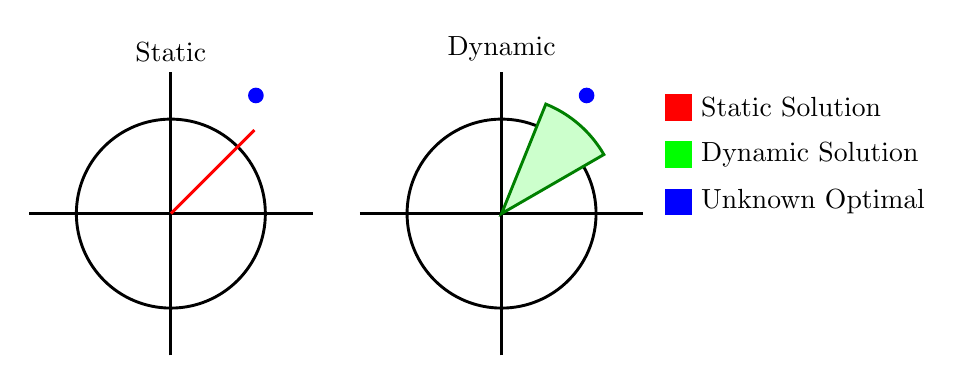
\begin{tikzpicture}[scale=0.6, line width=1.05][]

	\node at (0.0 , 1) [above] {Static};
    \draw (-3.0,  -2.0) -- ( 3.0,  -2.0);
	\draw ( 0.0, -5.0) -- ( 0.0,  1.0);
	\draw ( 0.0,  -2.0) circle [radius=2cm];
	\node[blue] at (1.8, 0.5) [circle, fill, inner sep=2pt]{};
	\draw[red] (0.0, -2.0) -- ++(45:2.5);

	\node at (7.0 , 1) [above] {Dynamic};
    \draw ( 4.0,  -2.0) -- (10.0, -2.0);
	\draw ( 7.0, -5.0) -- ( 7.0, 1.0);
	\draw ( 7.0,  -2.0) circle [radius=2cm];
	\node[blue] at (8.8, 0.5) [circle, fill, inner sep=2pt]{};
	\filldraw[fill=green!20,draw=green!50!black] (7,-2) -- ++(30:2.5cm)
	        arc [start angle=30, end angle=68, radius=2.5cm] -- cycle;

	
	\begin{scope}[shift={(10.5,0.5)}]
		% \node at (-0.25,1) [right] {};
		\draw[color=red,fill] (0,0.0)  rectangle  (0.5, -0.5);
		\node[anchor=west] at (0.5, -0.25) { Static Solution};

		\draw[color=green,fill] (0,-1.0)  rectangle  (0.5, -1.5);
		\node[anchor=west] at (0.5, -1.25) { Dynamic Solution};

		\draw[color=blue,fill] (0,-2.0)  rectangle  (0.5, -2.5);
		\node[anchor=west] at (0.5, -2.25) { Unknown Optimal};
	\end{scope}

    % \shade[ball color=red!50!white,opacity=0.8] (0,0) -- (90:\radius) arc (90:-90:\height) -- cycle;

	\end{tikzpicture}
}


    \end{block}
\end{frame}

\begin{frame}{}
    \begin{block}{Business}
		\usetikzlibrary{positioning}
\definecolor{red}{HTML}{8A3F3A}
\definecolor{yellow}{HTML}{E0BB3C}
\definecolor{blue}{HTML}{4569E0}
\definecolor{green}{HTML}{17E561}
\definecolor{other}{HTML}{6A939E}

% DTU Colors
\definecolor{dtu-corporate-red}{HTML}{990000}
\definecolor{dtu-white}{HTML}{ffffff}
\definecolor{dtu-black}{HTML}{000000}
\definecolor{dtu-blue}{HTML}{2F3EEA}
\definecolor{dtu-bright-green}{HTML}{1FD082}
\definecolor{dtu-navy-blue}{HTML}{030F4F}
\definecolor{dtu-yellow}{HTML}{F6D04D}
\definecolor{dtu-orange}{HTML}{FC7634}
\definecolor{dtu-pink}{HTML}{F7BBB1}
\definecolor{dtu-grey}{HTML}{DADADA}
\definecolor{dtu-red}{HTML}{E83F48}
\definecolor{dtu-green}{HTML}{008835}
\definecolor{dtu-purple}{HTML}{79238E}


\newlength{\basisa}
\setlength{\basisa}{1cm}
\centering
\begin{tikzpicture}[line width=0.0\basisa]
    \draw (4.0\basisa,4.0\basisa) 
		node[minimum height=2\basisa,fill=dtu-grey,minimum width=3\basisa,rounded corners=0.1\basisa] 
			(Planner) {Planner};
    \draw (12.0\basisa,4.0\basisa) 
		node[minimum height=2\basisa,fill=dtu-grey,minimum width=3\basisa,rounded corners=0.1\basisa] 
			(Supervisor) {Supervisor};

			
    \draw (8.0\basisa,4.0\basisa) 
		node[minimum height=2\basisa,fill=dtu-green,minimum width=3\basisa,rounded corners=0.1\basisa] 
			(Scheduler) {Scheduler};
	
    \draw (8.0\basisa,1.5\basisa) 
		node[minimum height=1\basisa,fill=dtu-blue,minimum width=3\basisa,rounded corners=0.1\basisa] 
			(Database) {Database};

    \draw (8.0\basisa,6.5\basisa) 
		node[minimum height=1\basisa,fill=dtu-yellow,minimum width=3\basisa,rounded corners=0.1\basisa] 
			(UserInterface) {User Interface};

	\draw[<->, thick, line width=0.1\basisa] (Planner) -- (Scheduler);
	\draw[<->, thick, line width=0.1\basisa] (Scheduler) -- (Supervisor);
	\draw[<->, thick, line width=0.1\basisa] (Scheduler) -- (Database);
	\draw[<->, thick, line width=0.1\basisa] (Scheduler) -- (UserInterface);
\end{tikzpicture}

		% Business usually handle decision making by making a series of "model changes" which 
		% are then combined to create a decision process.
  %       \begin{enumerate}
  %       \end{enumerate}
    \end{block}
\end{frame}

\end{document}
